\documentclass[11pt, a4paper, spanish]{article}

\usepackage[a4paper, margin=2.5cm, top=3.5cm, bottom=3.5cm]{geometry} % Define los márgenes
\usepackage{amsmath, amscd, amssymb, amsthm, latexsym, gensymb} % Paquetes matemáticos
\usepackage[spanish]{babel} % Traduce los paquetes a español
\usepackage[utf8]{inputenc} % Codificación UTF8
\usepackage{fancyhdr} % Encabezados y pies de página
  \pagestyle{fancyplain}
\usepackage{enumerate}
\usepackage{xspace}
\usepackage[page, toc]{appendix} % Apéndices
\usepackage[nottoc]{tocbibind} % Referencias en la TDC
\usepackage{scrextend} % Para usar addmargin
\usepackage{listings} % Código
  \lstdefinestyle{customcpp}{
    belowcaptionskip=1\baselineskip,
    breaklines=true,
    xleftmargin=3em,
    language=C++,
    basicstyle=\small\ttfamily
  }
\usepackage[onelanguage, spanish]{algorithm2e}
  % \NoCaptionOfAlgo
  \LinesNumbered\RestyleAlgo{ruled}\IncMargin{1em}\DontPrintSemicolon\SetArgSty{}\SetCommentSty{textsf}\SetFuncSty{textsf}
  \SetKwProg{For}{para}{ hacer}{fin}
  \SetKwProg{Fn}{función}{:}{fin}
\usepackage[pdftex]{graphicx} % Imágenes
\usepackage[usenames,dvipsnames]{color} % Autoexplicativo
\usepackage{caption} % Captions sin números
\usepackage{caratula} % Carátula del DC

% Bibliografía
\usepackage{biblatex}
\addbibresource{referencias.bib}

% Comandos personalizados
\let\strong\textbf
\renewcommand{\appendixtocname}{Apéndices}
\renewcommand{\appendixpagename}{Apéndices}
\theoremstyle{plain}
  \newtheorem{prop}{Proposición}
  \newtheorem{lema}{Lema}
\theoremstyle{remark}
  \newtheorem{obs}{Observación}
\setlength{\parskip}{.3em}

% Encabezado
\lhead{Métodos Numéricos}
\rhead{Trabajo Práctico Nº 1 - \emph{``Con 15 $\theta$s discretizo alto horno''}}
% Pie de pagina
\renewcommand{\footrulewidth}{0.4pt}
% \lfoot{FCEN}
% \rfoot{UBA}

\begin{document}

% Datos de carátula
\materia{Métodos Numéricos}
\titulo{Trabajo Práctico Nº 1}
\subtitulo{``Con 15 $\theta$s discretizo alto horno''}
\fecha{Segundo cuatrimestre de 2015}

\integrante{Frizzo, Franco}{013/14}{francofrizzo@gmail.com}
\integrante{Martínez, Manuela}{160/14}{martinez.manuela.22@gmail.com}
\integrante{Rabinowicz, Lucía}{105/14}{lu.rabinowicz@gmail.com}

% Carátula
\maketitle
\newpage

% Resumen y palabras clave
\begin{addmargin}[4em]{4em}

\section*{\centering Resumen}
  {\color{Gray} El resumen, de no más de 200 palabras, deberá explicar brevemente el trabajo realizado y las conclusiones de los autores de manera que pueda ser útil por sí solo para dar una idea del contenido del trabajo.}

\vspace{4em}
\noindent \strong{Palabras clave:} {\color{Gray} Las palabras clave, no más de cuatro, deben ser términos técnicos que den una idea del contenido del trabajo para facilitar su búsqueda en una base de datos temática.}

\end{addmargin}
\clearpage

% Índice
\tableofcontents
\clearpage

% Contenido
\section{Introducción teórica}

  {\color{Gray} Contendrá una breve explicación de la base teórica que fundamenta los métodos involucrados en el trabajo, junto con los métodos mismos. No deben incluirse demostraciones de propiedades ni teoremas, ejemplos innecesarios, ni definiciones elementales (como por ejemplo la de matriz simétrica). En vez de definiciones básicas es conveniente citar ejemplos de bibliografía adecuada. \emph{Una cita vale más que mil palabras.}}

  En el presente trabajo, nos proponemos utilizar un modelo matemático para resolver un problema físico. Consideraremos la sección horizontal de un alto horno, que es un horno cilíndrico en cuyo interior se realiza la fusión de metales a temperaturas muy elevadas. Se conocen la temperatura en la pared interior del horno, que es constante y de 1500{\degree}C, y se cuenta con sensores que proporcionan información sobre la temperatura en el exterior del horno, que oscila entre 50 y 200{\degree}C. Con el objeto de evaluar la peligrosidad de la estructura, resulta útil calcular la posición de la isoterma de 500{\degree}C en el interior de la pared, y contar con un criterio que permita decidir, en función al resultado obtenido, si existe algún riesgo de colapso de la estructura.

  \begin{figure}[h]
    \centering
    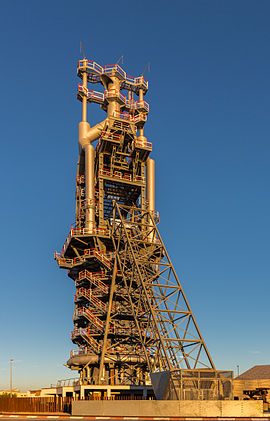
\includegraphics[width=4cm]{altoHorno.jpg}
    \caption{Alto horno.}
  \end{figure}

  Contamos con un modelo matemático, que explicaremos con más detalle en la próxima sección, que nos permite discretizar el dominio del problema y resolverlo por medio de un sistema de ecuaciones lineales. Por lo tanto, serán de interés para nosotros los métodos que permitan encontrar soluciones de este tipo de sistemas de manera computacional.

  Utilizaremos dos métodos diferentes para encarar el problema planteado: el método de Eliminación Gaussiana y el de Factorización LU. Ambos se valen del hecho de que un sistema de ecuaciones puede expresarse en forma matricial, y de que realizando ciertas operaciones sobre las filas de la matriz del sistema, puede obtenerse un sistema equivalente, que tiene las mismas soluciones. Más aún, puede probarse que todo sistema es equivalente a otro cuya matriz es triangular, y encontrar la solución de este tipo de sistemas es sumamente sencillo, utilizando los algoritmos de sustitución hacia adelante o sustitución hacia atrás.

  El método de \emph{Eliminación Gaussiana} itera sobre las columnas de la matriz, colocando ceros en todas las posiciones que se encuentran por debajo de la diagonal. Para hacer esto, en la $i$-ésima iteración, se resta a todas las filas a partir de la $i + 1$ un múltiplo de la fila $i$-ésima, con un factor elegido convenientemente. Esto asegura que, al completar el algoritmo, la matriz obtenida será triangular superior.

  En su forma más básica, el método falla si en alguna iteración se anula el elemento de la diagonal correspondiente a la columna sobre la que se está trabajando. Para salvar esta dificultad, se utiliza una técnica conocida como \emph{pivoteo}, que consiste en alterar el orden de las filas o de las columnas de la matriz. Sin embargo, como probaremos más adelante, la matriz asociada al sistema que estudiaremos tiene la particularidad de que el algoritmo de Eliminación Gaussiana puede aplicarse sin realizar pivoteo.

  El método de \emph{Factorización LU}, por su parte, aprovecha el hecho de que bajo ciertas condiciones, una matriz $A$ puede factorizarse como el producto de otras dos, en la forma $A = LU$, donde $L$ es triangular inferior con unos en la diagonal, y $U$ es triangular superior. De esta manera, el sistema $Ax=b$ puede reescribirse como $LUx=b$, y luego ser resuelto en dos etapas sencillas: si llamamos $y=Ux$, podemos resolver primero el sistema $Ly=b$ (aplicando sustitución hacia adelante, pues $L$ es triangular inferior), y una vez conocido el valor de $y$, resolver $Ux=y$ (aplicando esta vez sustitución hacia atrás), obteniendo así la solución del sistema original.

\clearpage
\section{Desarrollo}

  {\color{Gray} Deben explicarse los métodos numéricos que utilizaron y su aplicación al problema concreto involucrado en el trabajo práctico. Se deben mencionar los pasos que siguieron para implementar los algoritmos, las dificultades que fueron encontrando y la descripción de cómo las fueron resolviendo. Explicar también cómo fueron planteadas y realizadas las mediciones experimentales. Los ensayos fallidos, hipótesis y conjeturas equivocadas, experimentos y métodos malogrados deben figurar en esta sección, con una breve explicación de los motivos de estas fallas (en caso de ser conocidas).}

  \subsection{Modelado y planteo del sistema}

    Llamamos $r_e \in \mathbb{R}_{>0}$ al radio exterior y $r_i \in \mathbb{R}_{>0}$ al radio interior de la pared del horno. Para cada punto, consideramos sus coordenadas polares $(r, \theta)$ con origen en el centro del horno, y llamaremos $T(r, \theta)$ a la temperatura en dicho punto. En el estado estacionario, esta temperatura satisface la ecuación del calor:

    \begin{equation} \label{des:eq:calor}
      \frac{\partial^2 T(r, \theta)}{\partial r^2} + \frac{1}{r} \frac{\partial T(r, \theta)}{\partial r} + \frac{1}{r^2} \frac{\partial^2 T(r, \theta)}{\partial \theta^2} = 0
    \end{equation}

    Para poder tratar computacionalmente el problema, necesitamos una versión discreta del mismo. Con este fin, consideramos una partición del sector interno de la pared del horno en $m + 1$ radios equidistantes, $r_i = r_0 < r_1 < \dots < r_m = r_e$, con $r_j - r_{j-1} = \Delta r$ para $j = 1, \dots m+1$, y en $n$ ángulos, $0 = \theta_0 < \theta_1 < ... < \theta_n = 2\pi$, con $\theta_k - \theta_{k-1} = \Delta \theta$ para $k = 1, \dots n$.

    Nuestro objetivo es calcular el valor de $t_{j,k} = T(r_j, \theta_k)$ para $j = 0, \dots m$ y $k = 0, \dots n-1$, utilizando la ecuación (\ref{des:eq:calor}) y los datos disponibles sobre las condiciones de borde: conocemos el valor de la temperatura en los puntos de la pared externa, $t_{m,k} = T_e(\theta_k)$, para todo $k = 0, \dots n-1$, como así también el valor de la temperatura en el interior del horno, $t_{0,k} = T_i$, que es constante con respecto a $k$.

    Para discretizar el problema continuo planteado por la ecuación (\ref{des:eq:calor}), utilizamos las siguientes fórmulas de diferencias finitas:
    \[ \frac{\partial^2 T(r, \theta)}{\partial r^2}(r_j, \theta_k) \cong \frac{t_{j-1,k} - 2 t_{jk} + t_{j+1,k}}{(\Delta r)^2} \]
    \[ \frac{\partial T(r, \theta)}{\partial r}(r_j, \theta_k) \cong \frac{t_{j,k} - t_{j-1,k}}{\Delta r} \]
    \[ \frac{\partial^2 T(r, \theta)}{\partial \theta^2}(r_j, \theta_k) \cong \frac{t_{j,k-1} - 2 t_{jk} + t_{j,k+1}}{(\Delta \theta)^2} \]
    que nos permiten obtener un conjunto de ecuaciones lineales en las incógnitas $t_{j,k}$.

    De esta manera, podemos reunir la información de la que disponemos sobre el problema discreto en un sistema de $(m+1)n$ ecuaciones con $(m+1)n$ incógnitas, cada una de ellas el valor de $t_{j,k}$ para algún $j = 0, \dots m$, $k = 0, \dots n-1$. En otras palabras, el problema de calcular la temperatura en todos los puntos de la discretización se reduce a la resolución del siguiente sistema de ecuaciones lineales:

    \begin{equation} \label{des:eq:sistema}
      \begin{cases}
      \setlength{\jot}{2em}
        t_{0,k} = T_i
          & \text{para } 0 \leq k < n \\[1em]
        \begin{gathered}
          \left( \frac{1}{(\Delta r)^2} - \frac{1}{r \Delta r} \right) t_{j-1,k} +
            \left( \frac{1}{r^2(\Delta \theta)^2} \right) t_{j,k-1} + \\
            \left( - \frac{2}{(\Delta r)^2} + \frac{1}{r \Delta r} - \frac{2}{r^2(\Delta \theta)^2} \right) t_{j,k} + \\
            \left( \frac{1}{r^2(\Delta \theta)^2} \right) t_{j,k+1} +
            \left( \frac{1}{(\Delta r)^2} \right) t_{j+1,k} = 0 \\[1em]
          \end{gathered}
          & \text{para } 1 \leq j < m,\ 0 \leq k < n \\
        t_{m,k} = T_e(\theta_k)
          & \text{para } 0 \leq k < n \\
      \end{cases}
    \end{equation}

    Para construir la matriz $A \in \mathbb{R}^{(m+1)n \times (m+1)n}$ asociada a este sistema, ordenamos las ecuaciones y las variables de la siguiente forma:
    \begin{itemize}
      \item La ecuación referida a la variable $t_{j,k}$, es decir, la ecuación donde aparece como única incógnita cuando $j = 0$ o $j = m$, o bien la ecuación donde aparece junto a sus cuatro puntos vecinos en la discretización si $1 \leq j < m$, es representada por la fila $p$-ésima de la matriz, con $p = jn+k$.
      \item A la variable $t_{j,k}$ le corresponde la columna $q$-ésima, con $q = jn+k$.
    \end{itemize}

    La matriz $A$ construida de esta forma cumple con la importante propiedad de ser \emph{banda} $n, n$. Esto significa que todos los coeficientes que se encuentran fuera de una banda de ancho $n$ hacia ambos lados de la diagonal son nulos, i.e. $A_{p,q} = 0$ siempre que $\vert p - q \vert > n$. Esto puede verse fácilmente:

    \begin{itemize}
      \item Las filas $1, \dots, n$ y $mn + 1, \dots, (m+1)n$ de la matriz, que corresponden a las ecuaciones relativas a los puntos de la pared interna y externa del horno, respectivamente, contienen un $1$ en la diagonal y $0$ en todas las demás posiciones, por lo que la propiedad se verifica trivialmente.
      \item Para $p = n + 1, \dots, mn$, la fila $p$-ésima de la matriz representa a la ecuación relativa a $t_{j,k}$, con $p = jn+k$. Es sencillo comprobar que los coeficientes correspondientes a $t_{j-1,k}$, $t_{j,k-1}$, $t_{j,k}$, $t_{j,k+1}$ y $t_{j+1,k}$ se encontrarán en las columnas $p-n$, $p-1$, $p$, $p+1$ y $p+n$, respectivamente. Estos elementos están confinados a una banda de ancho $n$ hacia ambos lados de la diagonal, y como las variables a las que corresponden son las únicas que aparecen en la ecuación, todos los demás coeficientes de la fila serán necesariamente nulos.
    \end{itemize}

  \subsection{Métodos utilizados}

    Los métodos numéricos que utlizaremos para resolver el sistema de ecuaciones expuesto serán los dos ya introducidos en la sección anterior de este trabajo: el método de \emph{Eliminación Gaussiana} (sin pivoteo) y el de \emph{Factorización LU}.

    \subsubsection{Aplicabilidad de los métodos elegidos}
       Los métodos elegidos para hallar la solución del problema no son aplicables en cualquier caso, sino que requieren que se satisfagan determinadas hipótesis. Sin embargo, en el caso particular del sistema que estamos estudiando, podemos demostrar una serie de resultados que nos aseguran que los métodos elegidos son aplicables.

      \begin{prop} \label{prop:La matriz es diagonal dominante}
        La matriz $A \in \mathbb{R}^{(m+1)n \times (m+1)n}$, correspondiente al sistema expuesto en (\ref{des:eq:sistema}), es diagonal dominante, de manera no estricta.
      \end{prop}

      \begin{proof} \ 
        \begin{itemize}
          \item Para las filas $1$ a $n$ de la matriz, correspondientes al borde interno de la discretización, y $mn + 1 $ a $(m+1)n$, correspondientes al borde externo, tenemos que
            \[ A_{p,q} = \begin{cases}
              1 & \text{si $p = q$} \\
              0 & \text{si $p \neq q$}
            \end{cases} \]
          Por lo tanto,
            \[ \vert A_{p,p} \vert = 1 \geq 0 = \sum_{\substack{q=1 \\ q \neq p}}^{(m+1)n} \vert A_{p,q} \vert \]

          \item Las filas $n + 1$ a $mn$ de la matriz corresponden a los puntos $t_{j,k}$ de la discretización con $1 \leq j < m$. En todos estos casos, encontramos solo 5 coeficientes no nulos en la $p$-ésima fila, siendo el que aparece en la diagonal el correspondiente a la variable $t_{j,k}$, y por lo tanto
            \[ \begin{split}
              \vert A_{p,p} \vert &= \left \vert - \frac{2}{(\Delta r)^2} + \frac{1}{r \Delta r} - \frac{2}{r^2 (\Delta \theta)^2} \right \vert \\
              &= \left \vert - \frac{1}{(\Delta r)^2} + \frac{1}{r \Delta r} - \frac{2}{r^2 (\Delta \theta)^2} - \frac{1}{(\Delta r)^2} \right \vert \\
              &= \left \vert - \frac{r - \Delta r}{r (\Delta r)^2} - \frac{2}{r^2 (\Delta \theta)^2} - \frac{1}{(\Delta r)^2} \right \vert \\
              &= \left \vert \frac{r - \Delta r}{r (\Delta r)^2} + \frac{2}{r^2 (\Delta \theta)^2} + \frac{1}{(\Delta r)^2} \right \vert
            \end{split} \]

          Teniendo en cuenta que
            \[ r - \Delta r = (r_i + j \Delta r) - \Delta r = r_i + (j - 1) \Delta r > 0\]
          dado que $r_i, \Delta r > 0$ y $j \geq 1$, es fácil notar que todos los términos que aparecen dentro del módulo son positivos, y por lo tanto
            \[ \vert A_{p,p} \vert = \frac{r - \Delta r}{r (\Delta r)^2} + \frac{2}{r^2 (\Delta \theta)^2} + \frac{1}{(\Delta r)^2} \]

          Por otro lado
            \[ \begin{split}
              \sum_{\substack{q=1 \\ q \neq p}}^{(m+1)n} \vert A_{p,q} \vert &= \left \vert \frac{1}{(\Delta r)^2} - \frac{1}{r \Delta r} \right \vert + 2 \left \vert \frac{1}{r^2 (\Delta \theta)^2} \right \vert + \left \vert \frac{1}{(\Delta r)^2} \right \vert \\
              &= \left \vert \frac{r - \Delta r}{r (\Delta r)^2} \right \vert + \frac{2}{r^2 (\Delta \theta)^2} + \frac{1}{(\Delta r)^2} \\
              &= \frac{r - \Delta r}{r (\Delta r)^2} + \frac{2}{r^2 (\Delta \theta)^2} + \frac{1}{(\Delta r)^2} = \vert A_{p,p} \vert
            \end{split} \]
        \end{itemize}

        De lo anterior, se sigue que
          \[ \vert A_{p,p} \vert \geq \sum_{\substack{q=1 \\ q \neq p}}^{(m+1)n} \vert A_{p,q} \vert \qquad \text{para todo $p = 1, \dots, (m+1)n$} \]
        es decir, $A$ es diagonal dominante de forma no estricta.
      \end{proof}

      \begin{obs}
        \label{obs:Diagonal de A sin ceros}
        Para todo $p = 1, \dots, (m+1)n$, $\vert A_{p,p} \vert > 0$, i.e. la diagonal de $A$ no contiene ceros.
      \end{obs}

      A continuación, probaremos un resultado que nos será útil: al realizar el primer paso de Eliminación Gaussiana sobre una matriz diagonal dominante, la matriz resultante también lo es.

      \begin{lema}
        \label{lema:EG conserva diagonal dominante}
        Sea $A^{(0)} = A \in \mathbb{R}^{n \times n}$ una matriz diagonal dominante, y $A^{(1)}$ el resultado de aplicar un paso de Eliminación Gaussiana (sin pivoteo) sobre $A$. Entonces $A^{(1)}$ es diagonal dominante.
      \end{lema}
      \begin{proof}
        Consideremos la fila $i$-ésima de $A^{(1)}$, y veamos que $\left \vert A^{(1)}_{i,i} \right \vert \geq \sum_{\substack{j = 1 \\ j \neq i}}^n \left \vert A^{(1)}_{i,j} \right \vert$. Tenemos que
        \[ \left \vert A^{(1)}_{i,i} \right \vert = \left \vert A_{i,i} - \frac{A_{i,1}}{A_{1,1}} A_{1,i} \right \vert
          \qquad \text{y} \qquad
        \sum_{\substack{j = 1 \\ j \neq i}}^n \left \vert A^{(1)}_{i,j} \right \vert
          = \sum_{\substack{j = 2 \\ j \neq i}}^n \left \vert A_{i,j} - \frac{A_{i,1}}{A_{1,1}} A_{1,j} \right \vert \]

        Luego,

        \[ \begin{split}
          \sum_{\substack{j = 1 \\ j \neq i}}^n \left \vert A^{(1)}_{i,j} \right \vert
          &= \sum_{\substack{j = 2 \\ j \neq i}}^n \left \vert A_{i,j} - \frac{A_{i,1}}{A_{1,1}} A_{1,j} \right \vert \\
          &\leq \sum_{\substack{j = 2 \\ j \neq i}}^n \vert A_{i,j} \vert + \left \vert \frac{A_{i,1}}{A_{1,1}} \right \vert \sum_{\substack{j = 2 \\ j \neq i}}^n \vert A_{1,j} \vert \\
          &\leq \left( \vert A_{i,i} \vert - \vert A_{i,1} \vert \right) + \left \vert \frac{A_{i,1}}{A_{1,1}} \right \vert \left( \vert A_{1,1} \vert - \vert A_{1,i} \vert \right) \\
          &= \vert A_{i,i} \vert - \left \vert \frac{A_{i,1}}{A_{1,1}} \right \vert \vert A_{1,i} \vert \\
          &\leq \left \vert A_{i,i} -  \frac{A_{i,1}}{A_{1,1}} A_{1,i} \right \vert = \left \vert A^{(1)}_{i,i} \right \vert \qedhere
        \end{split} \]
      \end{proof}

      Nos gustaría demostrar que tanto el método de Eliminación Gaussiana (sin pivoteo) como el de Factorización LU son aplicables en el sistema estudiado. Sin embargo, gracias al siguiente resultado, sabemos que basta con probar que podemos aplicar el primero de ellos, lo cual mostraremos inmediatamente después.

      \begin{prop} \label{prop:EG sin pivoteo implica LU}
        Si el sistema $Ax=b$ puede ser resuelto aplicando Eliminación Gaussiana sin pivoteo, entonces la matriz $A$ puede ser factorizada de la forma $A=LU$, donde $U$ es una matriz triangular superior y $L$ es una matriz triangular inferior con unos en la diagonal.\cite[p.~403]{burden}
      \end{prop}

      \begin{prop} \label{prop:Puede aplicarse EG}
        Sea $Ax=b$ la representación matricial correspondiente al sistema expuesto en (\ref{des:eq:sistema}), con $A \in \mathbb{R}^{(m+1)n \times (m+1)n}$ y $b \in \mathbb{R}^{(m+1)n}$ construidos de la manera arriba explicada. Entonces, el sistema $Ax=b$ puede ser resuelto aplicando Eliminación Gaussiana sin pivoteo.
      \end{prop}

      \begin{proof}
        Probaremos que para $u \leq (m+1)n$, es posible realizar $u$ iteraciones de Eliminación Gaussiana sobre $A$ sin pivoteo, y que luego de las mismas, la matriz $A^{(u)}$ resultante es diagonal dominante, con su fila $u + 1$ no nula. Lo haremos por inducción en $u$.

          \begin{itemize}
            \item[\textbf{C.B.}] Teniendo en cuenta que la primera fila de la matriz $A$ tiene necesariamente un $1$ en la diagonal y $0$ en las demás posiciones, se deduce trivialmente que es posible aplicar el primer paso de Eliminación Gaussiana sin realizar pivoteo, dado que $A_{1, 1}$ es no nulo. Del Lema \ref{lema:EG conserva diagonal dominante}, se sigue que la matriz $A^{(1)}$ obtenida será diagonal dominante. Como $A_{1, 2} = 0$, tendremos $A^{(1)}_{2,2} = A_{2,2}$, que es necesariamente no nulo (Observación \ref{obs:Diagonal de A sin ceros}), por lo que la segunda fila de $A^{(1)}$ será no nula.
                
            \item[\textbf{P.I.}] Supongamos que la matriz $A^{(u - 1)}$, obtenida tras aplicar $u - 1$ pasos de Eliminación Gaussiana sobre $A$, es diagonal dominante, con su $u$-ésima fila no nula. Esto implica que $A^{(u - 1)}_{u,u} \neq 0$. Notemos que podemos escribir a $A^{(u - 1)}$ por bloques de la siguiente manera
              \[ A^{(u - 1)} = \left( \begin{matrix} U_{u - 1} & B \\ 0 & \widetilde{A}_{u - 1} \end{matrix} \right) \]
            donde las matrices $U_{u - 1} \in \mathbb{R}^{(u-1)\times(u-1)}$ y $\widetilde{A}_{u - 1} \in \mathbb{R}^{(n-u+1)\times(n-u+1)}$ son trivialmente diagonal dominantes.

            Podemos ver que realizar el paso $u$-ésimo del algoritmo de Eliminación Gaussiana sobre $A$ equivale a realizar el primer paso de este algoritmo sobre $\widetilde{A}_{u - 1}$, sin modificar el resto de la matriz. Dado que $A^{(u - 1)}_{u,u} \neq 0$, podremos realizar esto sin pivoteo, y del Lema 1 se sigue que el resultado de este proceso será diagonal dominante, lo cual implica directamente que también lo será $A^{(u)}$.

            Por último, probemos que la fila $u + 1$ de la matriz $A^{(u)}$ es no nula.
            \begin{itemize}
              \item Si $1 \leq u + 1 \leq n$ o $mn < u + 1 \leq (m+1)n$, tendremos que la fila $u + 1$ tendrá un $1$ en la diagonal y $0$ en las demás posiciones, por lo que no se verá afectada por el algoritmo de Eliminación Gaussiana. Luego $A^{(u)}_{u+1,u+1} = 1$.
              \item En caso contrario, por la forma en la que se construye la matriz del sistema, $A_{u+1,u+1+n}$ corresponde al coeficiente de la variable $t_{j,k+1}$ de la $u + 1$-ésima ecuación del sistema, que es trivialmente no nulo. Además, como notamos anteriormente, la matriz $A$ es \emph{banda} $n, n$. Por lo tanto, $A_{p,u+1+n} = 0$ para todo $p = 0, \dots, u$ y, por consiguiente, $A^{(u)}_{u+1,u+1+n} = A_{u+1,u+1+n}$. Esto implica que la fila $u + 1$ de la matriz $A^{(u)}$ es no nula, como queríamos probar. \qedhere
            \end{itemize}
          \end{itemize}
        \end{proof}

    \subsubsection{Algoritmos}

      \subsubsection*{Sustitución hacia adelante y sustitución hacia atrás}
        Como ya mencionamos anteriormente, los dos métodos a utilizar se basan en el hecho de que resolver un sistema de ecuaciones cuya matriz se encuentra en forma triangular (superior o inferior) es sumamente sencillo. Para lograrlo, se utilizan un par de algoritmos sencillos, el de \emph{sustitución hacia adelante} y el de \emph{sustitución hacia atrás}.

        El algoritmo de \emph{sustitución hacia adelante} considera un sistema de ecuaciones $Lx=b$, donde $L$ es una matriz triangular inferior, y devuelve un vector $s$ solución del sistema, con complejidad cuadrática en la cantidad de incógnitas. Lo hace aprovechando el hecho de que el valor de la primera incógnita puede ser despejado de forma inmediata; luego, sustituyendo este valor en la segunda ecuación, puede despejarse la segunda incógnita, y así sucesivamente hasta resolver el sistema completo. El pseudocódigo del algoritmo es el siguiente:

        \vspace*{1em}
        \begin{algorithm}[H]
          \caption{Sustitución hacia adelante}
          \SetKwFunction{sustAdelante}{Sustitución hacia adelante}
          \KwData{$A \in \mathbb{R}^{n \times n}, b \in \mathbb{R}^n$}
          \KwResult{$s \in \mathbb{R}^n$, solución del sistema $Ax=b$, considerando a $A$ como una matriz triangular inferior}
          \For{$i \gets 1$ \KwTo $n$}{
            $suma \gets 0$ \;
            \For{$j \gets 1$ \KwTo $i$}{
              $suma \gets suma + s_j \cdot A_{i,j}$ \;
            }
            $s_i \gets \frac{b_i - suma}{A_{i,i}}$
          }
        \end{algorithm}
        \vspace*{1em}

        El algoritmo de \emph{sustitución hacia atrás} es muy similar al anterior, pero considera un sistema de ecuaciones $Ux=b$, con $U$ triangular superior, y realiza el proceso recorriendo las filas de la matriz en orden inverso, desde abajo hacia arriba.

        \vspace*{1em}
        \begin{algorithm}[H]
          \SetKwFunction{sustAtras}{Sustitución hacia atrás}
          \caption{Sustitución hacia atrás}
          \KwData{$A \in \mathbb{R}^{n \times n}, b \in \mathbb{R}^n$}
          \KwResult{$s \in \mathbb{R}^n$, solución del sistema $Ax=b$, considerando a $A$ como una matriz triangular superior}
          \For{$i \gets n$ \KwTo $1$}{
            $suma \gets 0$ \;
            \For{$j \gets i + 1$ \KwTo $n$}{
              $suma \gets suma + s_j \cdot A_{i,j}$ \;
            }
            $s_i \gets \frac{b_i - suma}{A_{i,i}}$
          }
        \end{algorithm}
        \vspace*{1em}

      \subsubsection*{Eliminación Gaussiana}

        El algoritmo de \emph{Eliminación Gaussiana} permite resolver un sistema de ecuaciones encontrando otro sistema equivalente, pero en forma triangular superior, y luego aplicando el algoritmo de sustitución hacia atrás para hallar la solución del mismo.

        \begin{algorithm}[H]
          \caption{Eliminación Gaussiana}
          \KwData{$A \in \mathbb{R}^{n \times n}, b \in \mathbb{R}^n$}
          \KwResult{$s \in \mathbb{R}^n$, solución del sistema $Ax=b$}
          \For{$j \gets 1$ \KwTo $n$}{
            \For{$i \gets 1$ \KwTo $n$}{
              $m \gets \frac{A_{i,j}}{A_{j,j}}$ \;
              \For{$k \gets j$ \KwTo $n$}{
                $A_{i,k} \gets A_{i,k} - m \cdot A_{j,k}$ \;
              }
              $b_i \gets b_i - m \cdot b_j$ \;
            }
          }
          $s \gets$ \sustAtras{$A,b$} \;
        \end{algorithm}

      \subsubsection*{Factorización LU}

        El algoritmo de \emph{Factorización LU}.

        \begin{algorithm}[H]
          \caption{Factorización LU}
          \KwData{$A \in \mathbb{R}^{n \times n}$}
          \KwResult{$B \in \mathbb{R}^{n \times n}$, tal que los elementos ubicados por encima de y en la diagonal forman una matriz triangular superior $U$, y los ubicados por debajo de la misma, completados con unos en la diagonal, forman una matriz triangular inferior $L$, con $LU=A$}
          \For{$j \gets 1$ \KwTo $n$}{
            \For{$i \gets 1$ \KwTo $n$}{
              $m \gets \frac{A_{i,j}}{A_{j,j}}$ \;
              $B_{i}{j} \gets m$ \;
              \For{$k \gets j+1$ \KwTo $n$}{
                $B_{i,k} \gets A_{i,k} - m \cdot A_{j,k}$ \;
              }
            }
          }
        \end{algorithm}

    \subsubsection{Implementación}

  \subsection{Estimación de la posición de la isoterma y medida de la peligrosidad}

    Una vez obtenida la resolución del sistema, fue necesario decidir un criterio para estimar la ubicación de la isoterma pedida. Algunas de las alternativas que consideramos al respecto fueron las siguientes:

    \begin{itemize}
      \item Para cada ángulo $\theta_k$, considerar como posición de la isoterma el radio correspondiente al punto $(r_j, \theta_k)$ de la discretización con el valor de $t_{j,k}$ más próximo a 500{\degree}C.
      \item Para cada ángulo $\theta_k$, considerar como posición de la isoterma el radio del punto de la discretización inmediatamente exterior al primero con temperatura mayor o igual a 500{\degree}C, contando desde la pared externa. Es decir, considerar el menor radio $r_j$ tal que $t_{j',k} < 500$ para todo $j' \geq j$. La ventaja de este método es que asegura que la isoterma nunca se encontrará más cerca de la pared externa que el resultado arrojado, garantizando que se detectarán todas las posibles situaciones de riesgo.
      \item Para cada ángulo $\theta_k$, considerar $r_j$, el radio del punto más externo de la discretización con temperatura mayor o igual a 500{\degree}C. Luego, sabiendo que la isoterma buscada se encontrará entre este radio y el inmediatamente exterior, aproximar la variación de la temperatura en los puntos intermedios mediante una función lineal y utilizar esta aproximación para estimar la posición de la isoterma. Más precisamente, si $r_{iso}$ es el radio de la isoterma buscada, entonces
        \[ r_{iso} = r_j + \Delta r \left(\frac{500 - t_{j,k}}{t_{j+1,k} - t_{j,k}} \right) \]
    \end{itemize}

    Finalmente, decidimos aplicar este último criterio, porque consideramos que brinda información más precisa que los otros dos, al tener en cuenta el valor la diferencia de temperatura entre los puntos de la discretización más cercanos a la isoterma buscada y la isoterma en si misma, información que los dos primeros métodos descartan. De esta manera, nos permite detectar situaciones de riesgo que con el primer método pasarían desapercibidas, pero evitando la generación de falsos positivos que provocaría el segundo método, que es mucho más estricto.

    Para elegir la medida de peligrosidad lo que hacemos es tomar de todos los valores por los que pasa la isoterma el mas próximo a la pared externa del alto horno. A ese valor lo dividimos por el radio externo, dando así la relación entre la distancia mas cercana a la pared externa de la isoterma y la distancia total.
    Este es un numero entre 1 y 0 donde 0 es el centro del horno y 1 es la pared externa. Cuanto mas cercano a 1 sea el valor, mas peligro de colapsar tiene. 

  \subsection{Hipótesis planteadas}

    Suponemos que lo que va a pasar es que cuanto mas instancias haya en el sistema, mas diferencia va a haber entre los métodos numéricos a utilizar. El método de eliminación gaussiana es mas lento cuando aumentan las instancias ya que para cada una de ellas recalcula todo el sistema. En cambio, el método de factorización LU calcula la factorización LU del sistema una única vez y después modifica en base a este los parámetros de entrada para calcular el sistema total. Mientras que cuando hay pocas instancias el tiempo que tomarán va a ser muy similar. Eliminación gaussiana para una única instancia es un poco mas rápido que LU ya que no podemos sacar la ventaja de guardar la factorización LU para no recalcular la matriz del sistema cuando es un único sistema y a pesar de tener un orden similar, factorización LU supera a eliminación gaussiana por una constante.

  \subsection{Mediciones experimentales realizadas}

\clearpage
\section{Resultados}

  \subsubsection*{Experimento 1: Posición de la isoterma según granularidad}

    Para ambos casos se consideraron instancias de prueba con los siguientes parámetros: $r_i = 30$, $r_e = 60$, $T_i = 1500$, $iso = 500$. Se utilizó una temperatura externa constante en todos los puntos $(r_e, \theta)$ de la discretización, ($T_e(\theta) = 50$).

    En primer lugar, se calculó la solución del sistema y la posición estimada de la isoterma para una discretización considerablemente granular, con $m + 1 = 70$ y $n = 90$, para utilizar como caso de contraste. Reproducimos los gráficos que representan las temperaturas calculadas para todos los puntos de la discretización y la ubicación estimada de la isoterma.

    {\centering \begin{tabular}{cc}
      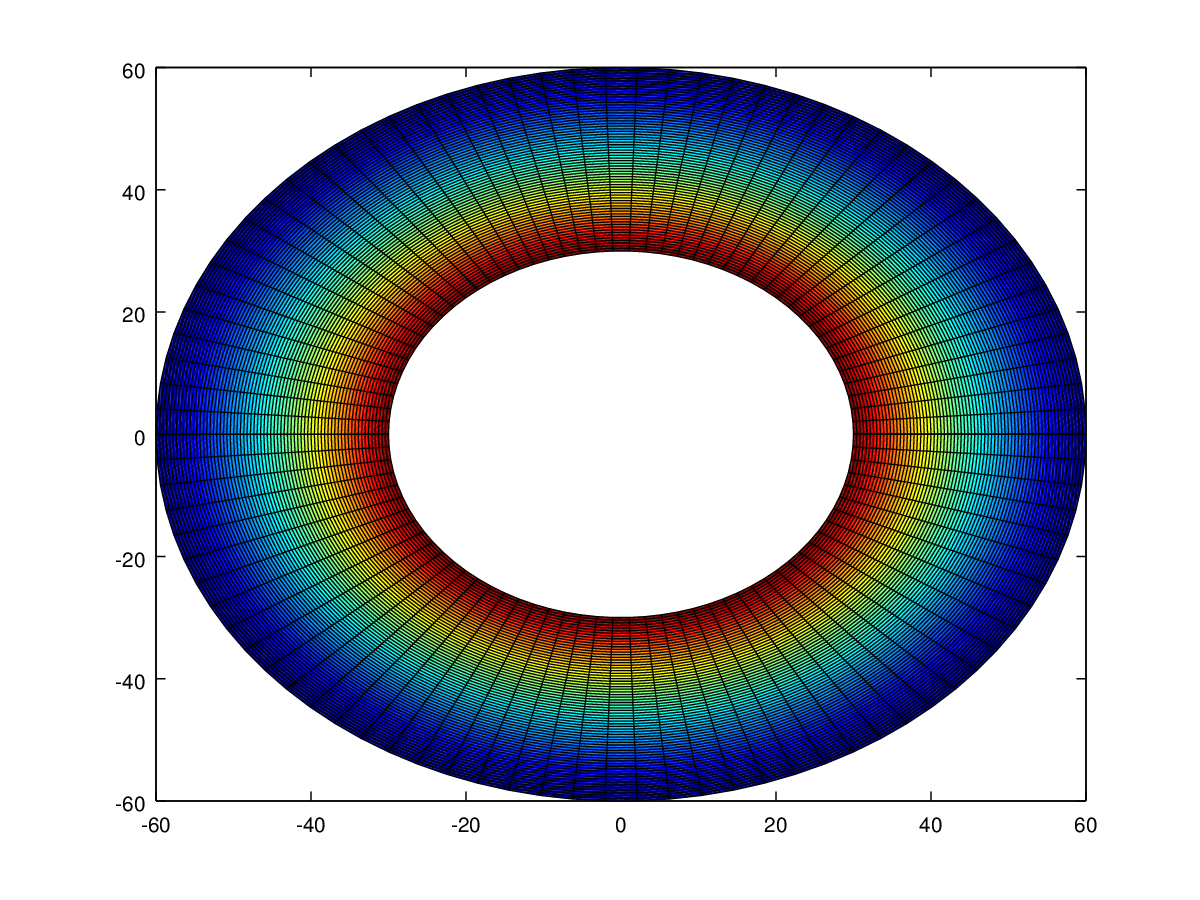
\includegraphics[height=5cm]{graficos/1/1-real.png} & 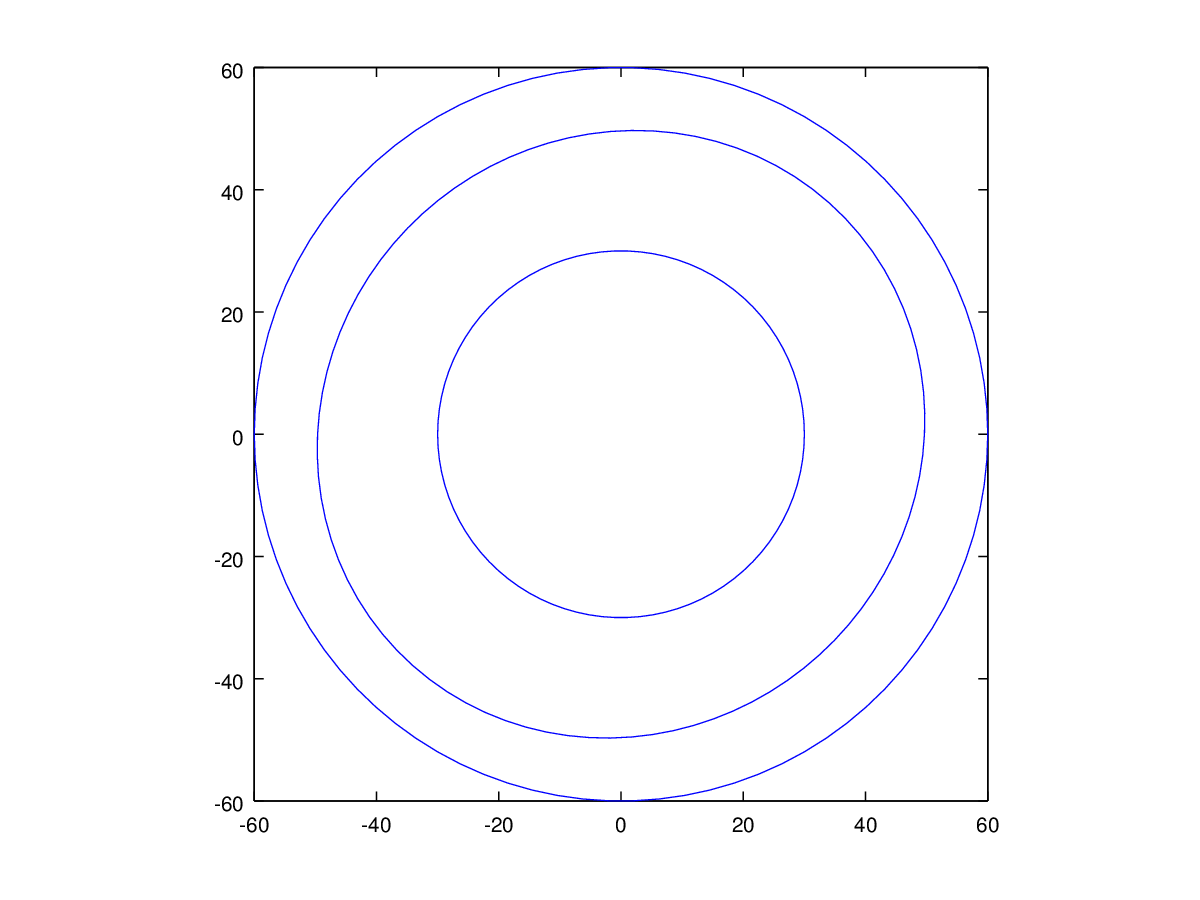
\includegraphics[height=5cm]{graficos/1/1-real-iso.png} \\
      {\small Temperaturas obtenidas} &
      {\small Posición estimada de la isoterma 500{\degree}C} \\
    \end{tabular}}

    \paragraph{Caso A} Se mantuvo constante la cantidad de radios de la discretización $m + 1 = 70$, y se tomaron instancias con diferentes cantidades de ángulos, para $n = 3, 5, 8, 10, 30, 50, 70$. Los gráficos que incluimos representan los resultados obtenidos para $n = 5, 10, 50$, reflejando las temperaturas calculadas y la ubicación estimada de la isoterma (en azul), comparada con la obtenida para el caso de contraste (en verde).

    {\centering \begin{tabular}{ccc}
      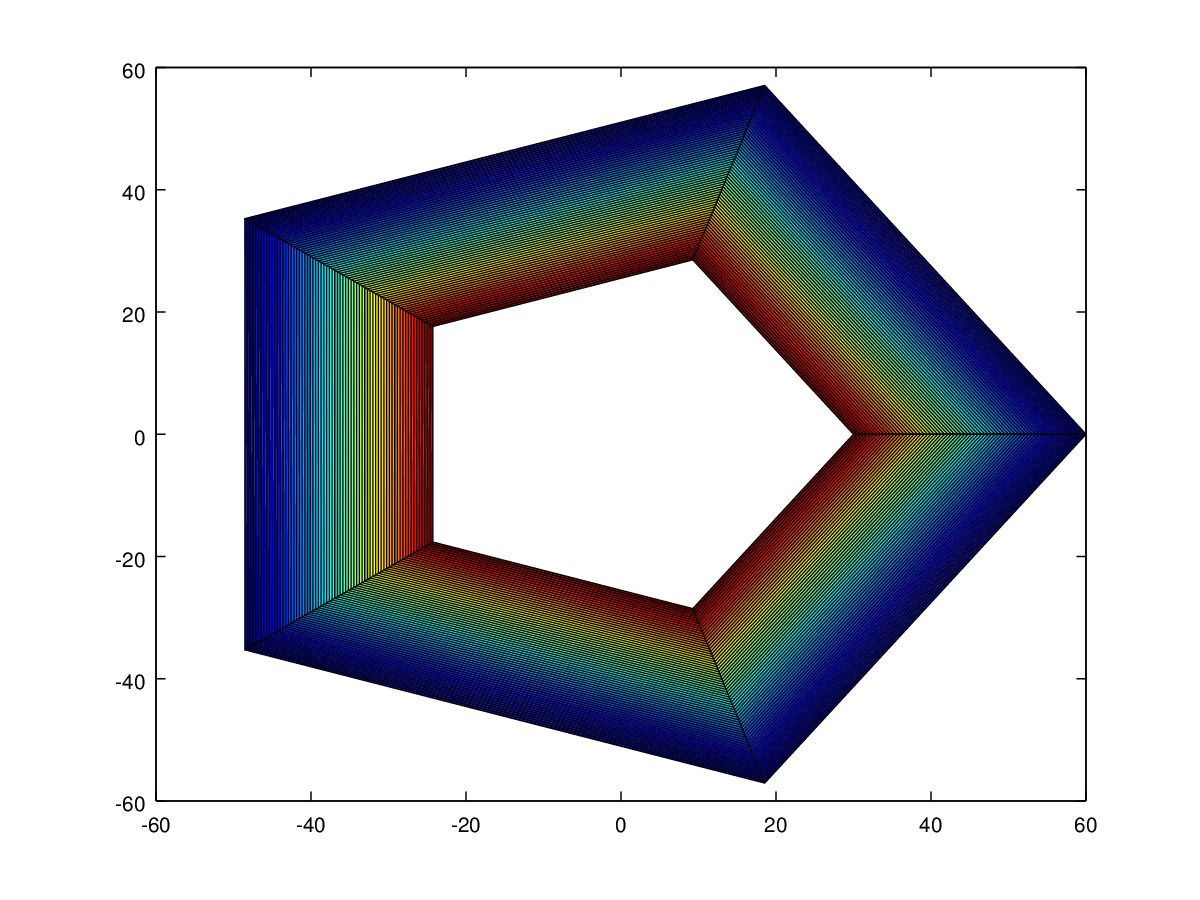
\includegraphics[width=4.5cm]{graficos/1/1a-5.png} &
      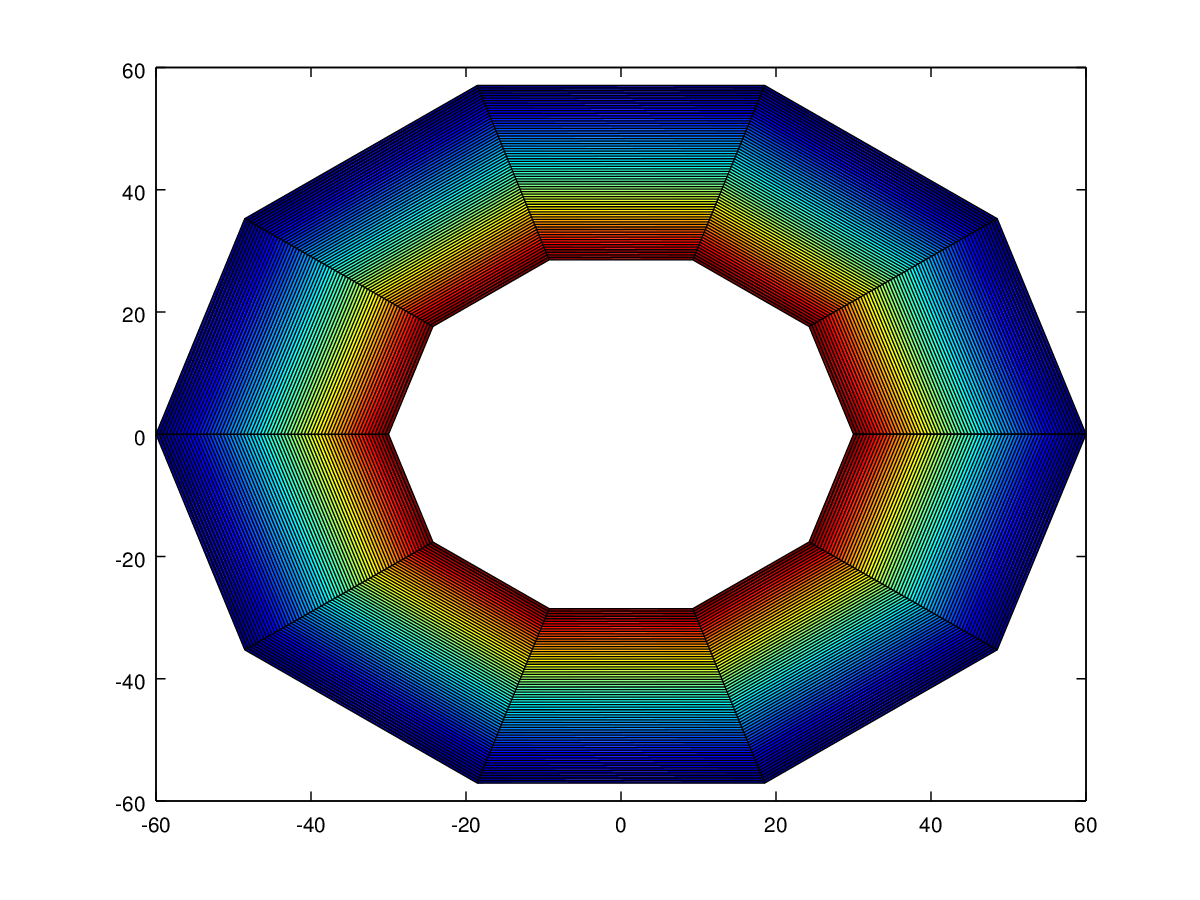
\includegraphics[width=4.5cm]{graficos/1/1a-10.png} &
      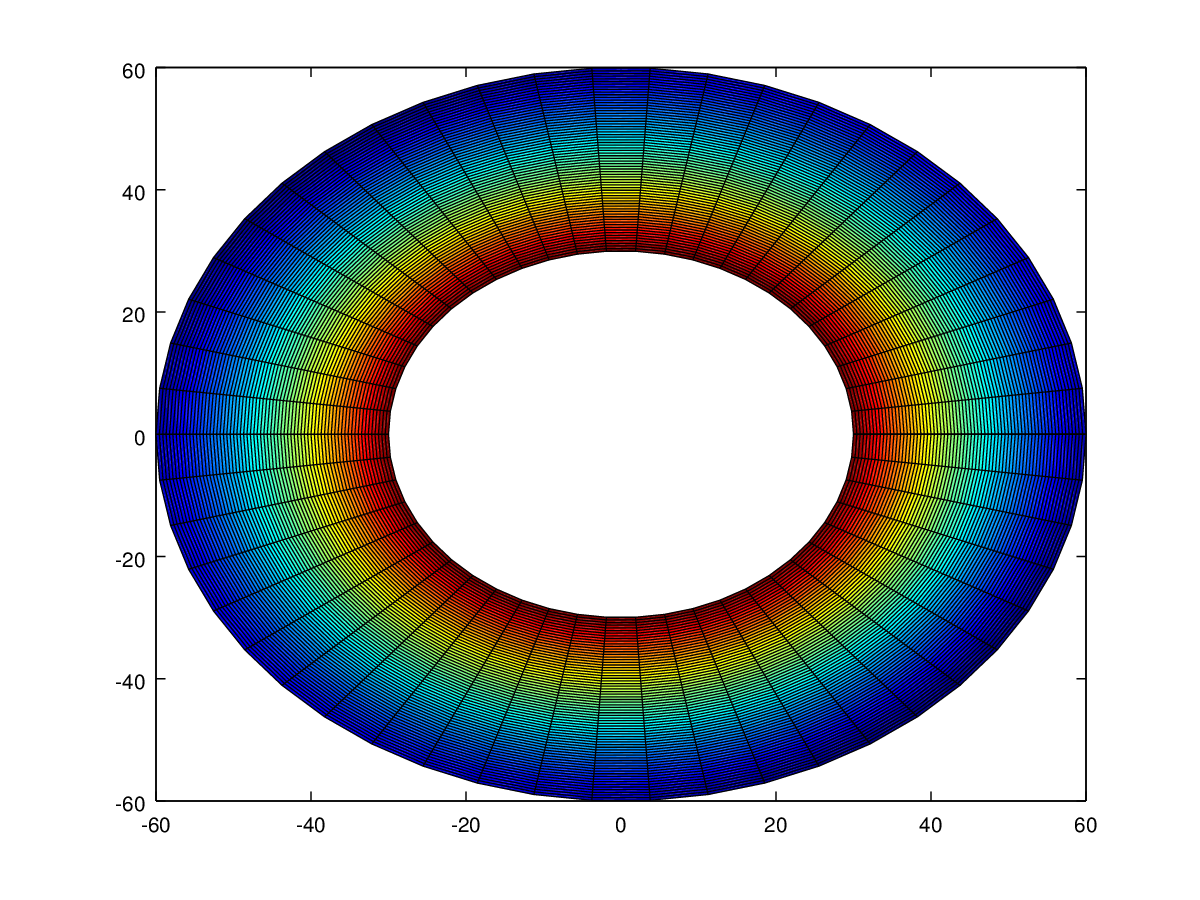
\includegraphics[width=4.5cm]{graficos/1/1a-50.png} \\
      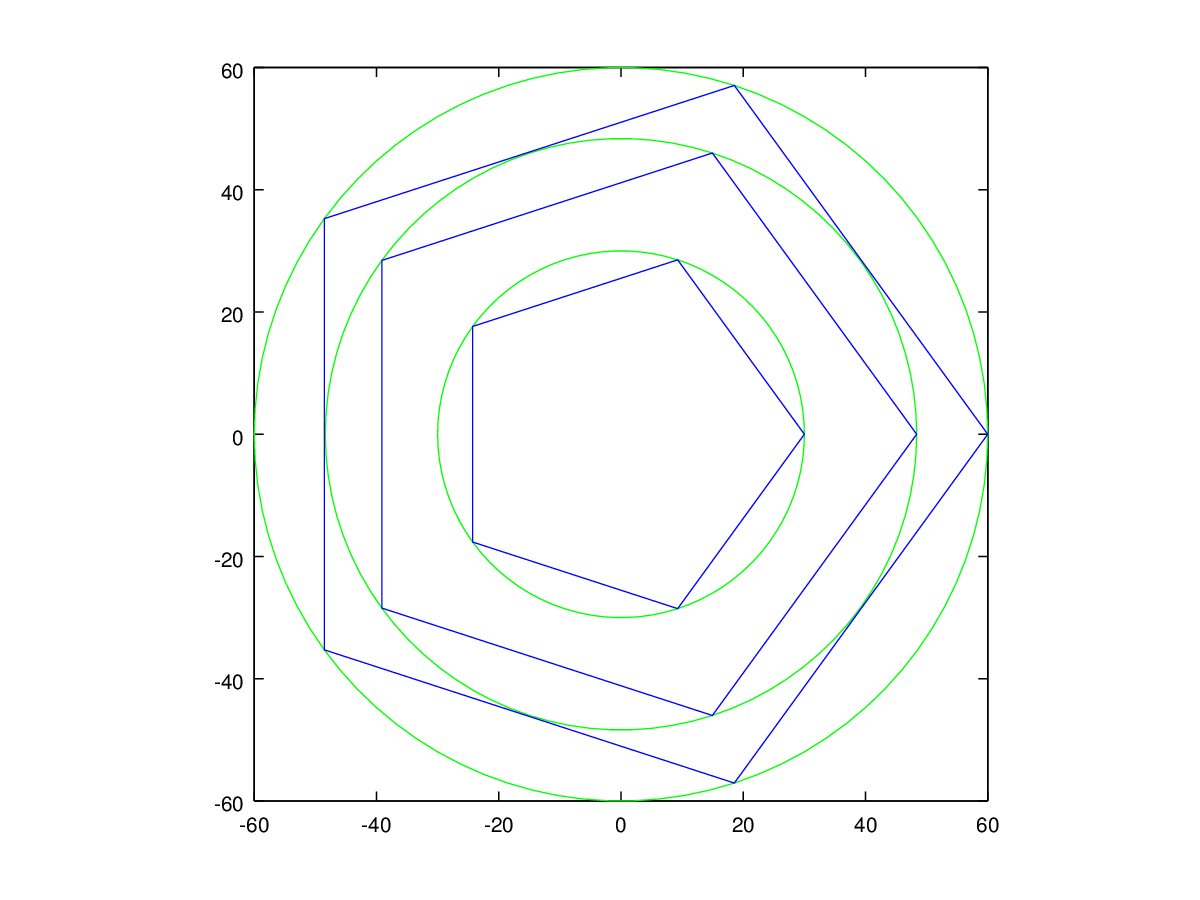
\includegraphics[width=4.5cm]{graficos/1/1a-5-iso.png} &
      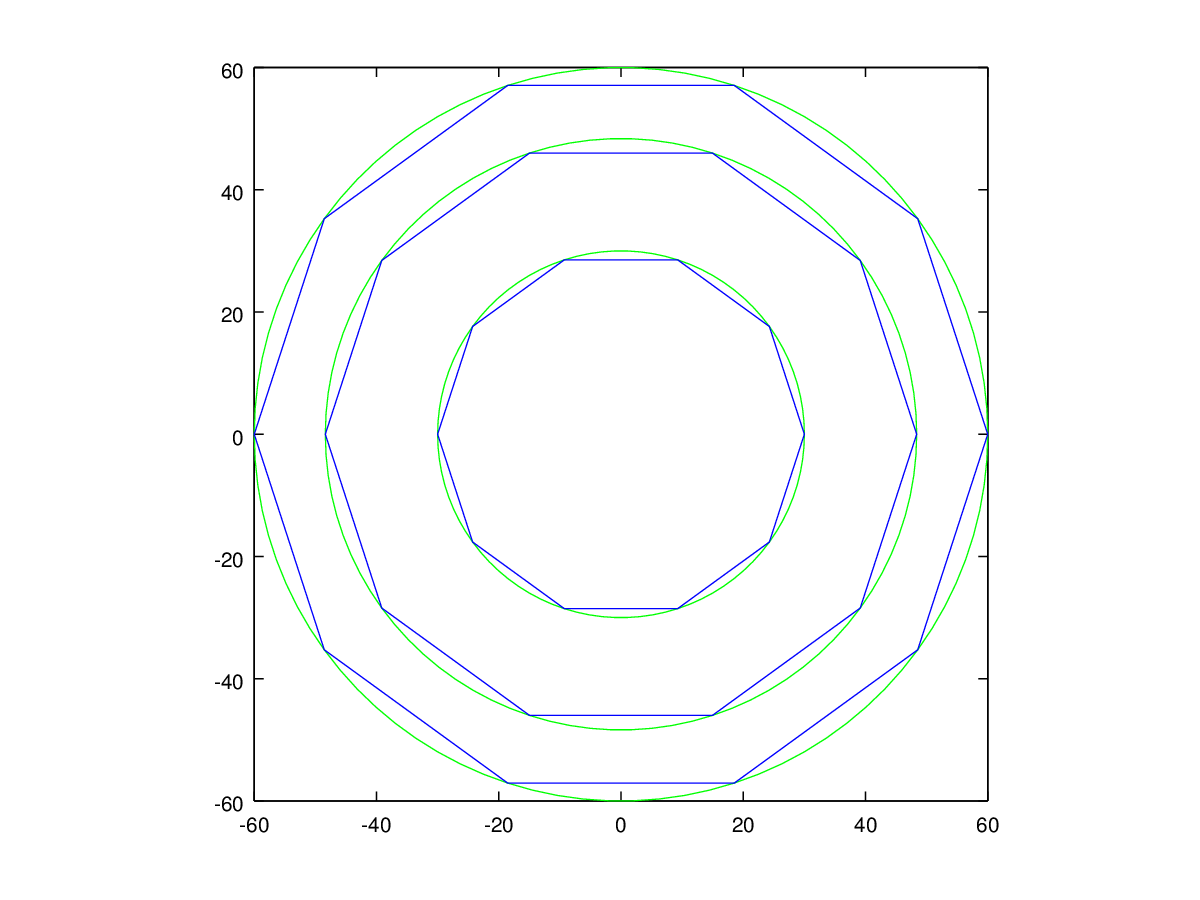
\includegraphics[width=4.5cm]{graficos/1/1a-10-iso.png} &
      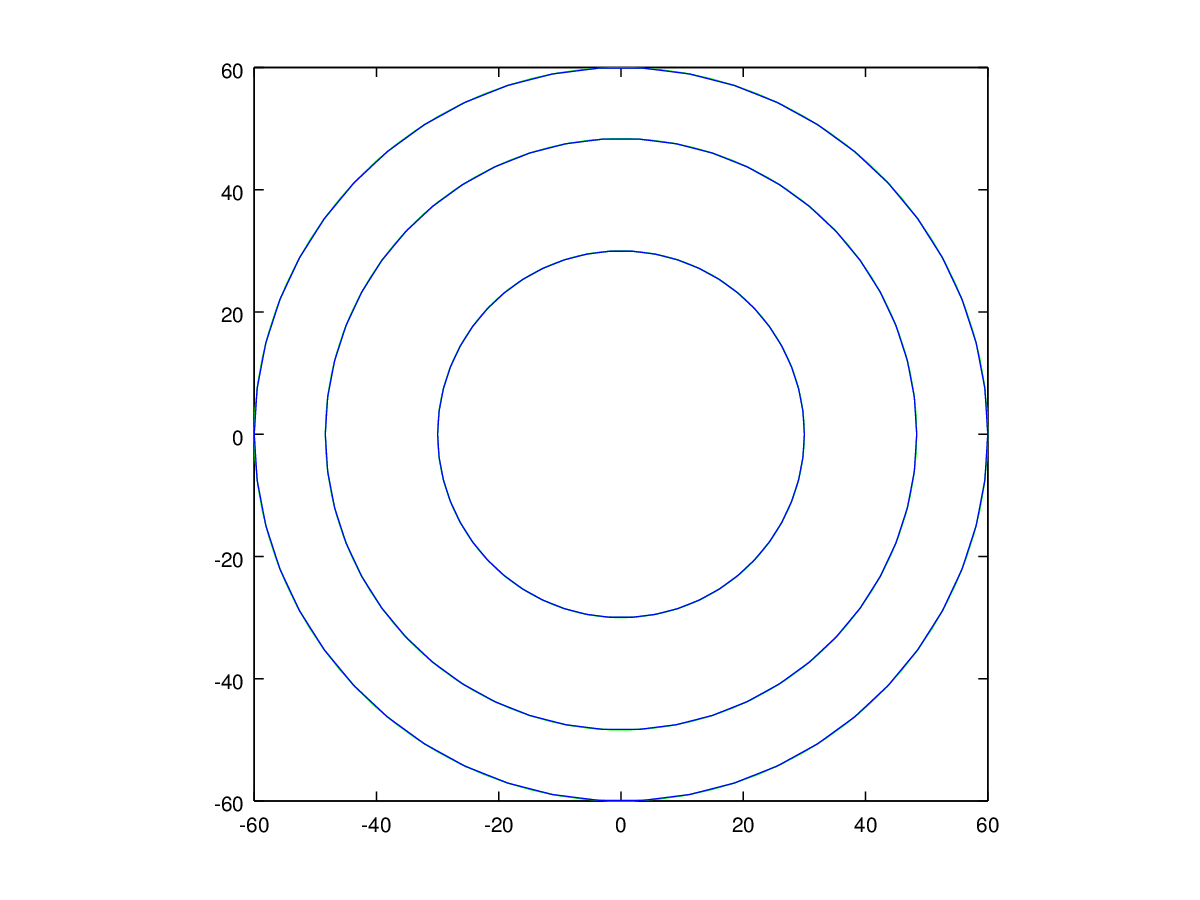
\includegraphics[width=4.5cm]{graficos/1/1a-50-iso.png} \\
      {\small $n = 5$} &
      {\small $n = 10$} &
      {\small $n = 50$} \\
    \end{tabular}}

    \paragraph{Caso B} Se mantuvo constante la cantidad de ángulos de la discretización $n = 90$, y se tomaron instancias con diferentes cantidades de ángulos, para $m + 1 = 3, 5, 8, 10, 30, 50$. Los gráficos que incluimos representan los resultados obtenidos para $m + 1 = 3, 8, 30$, reflejando las temperaturas calculadas y la ubicación estimada de la isoterma (en azul), comparada con la obtenida para el caso de contraste (en verde).

    {\centering \begin{tabular}{ccc}
      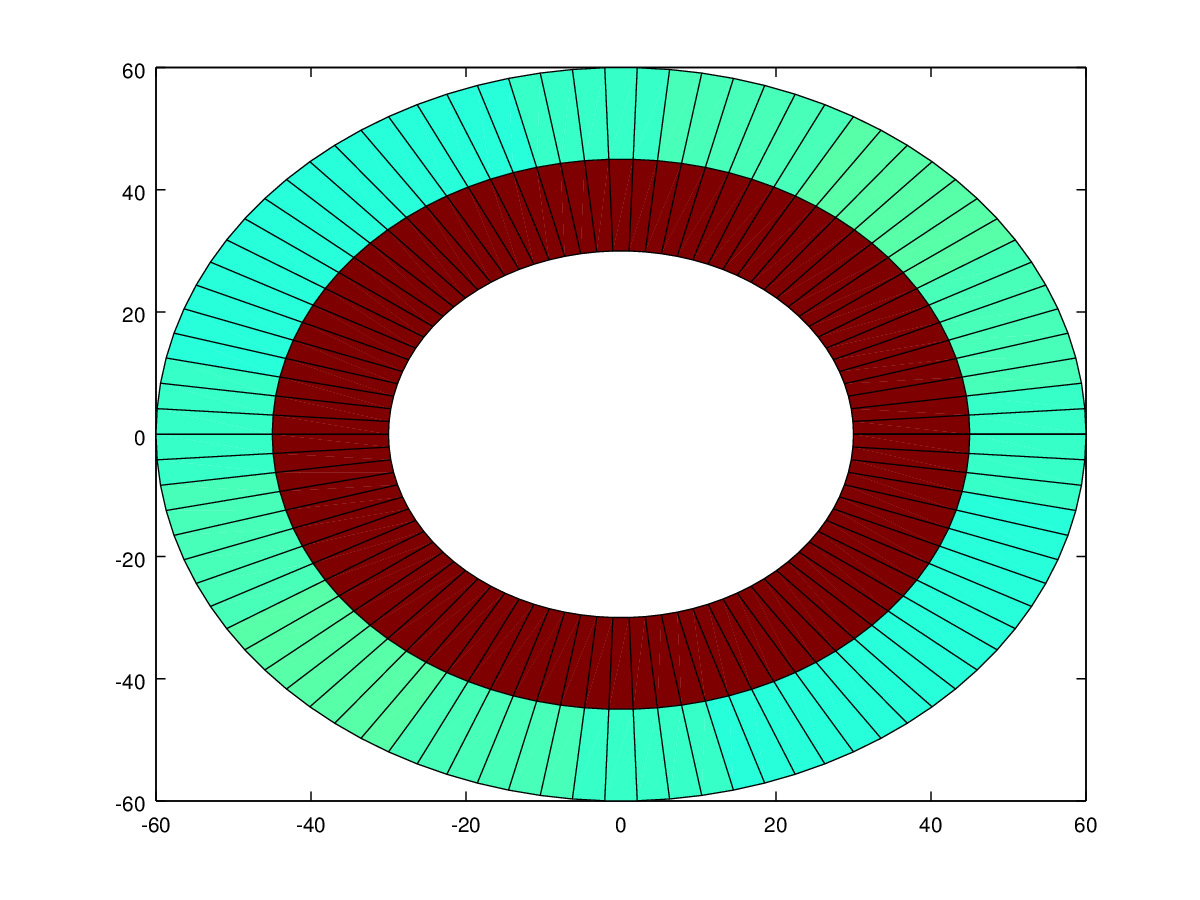
\includegraphics[width=4.5cm]{graficos/1/1b-3.png} &
      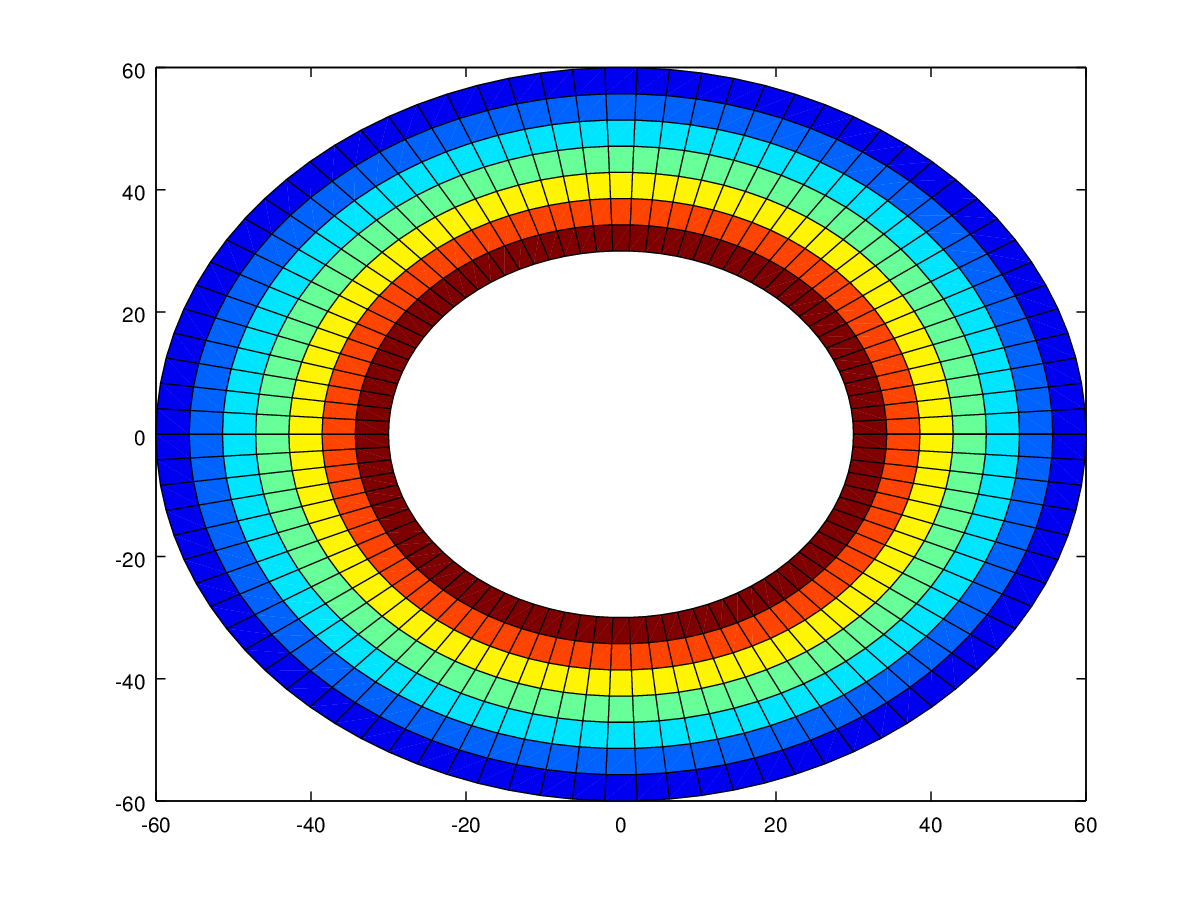
\includegraphics[width=4.5cm]{graficos/1/1b-8.png} &
      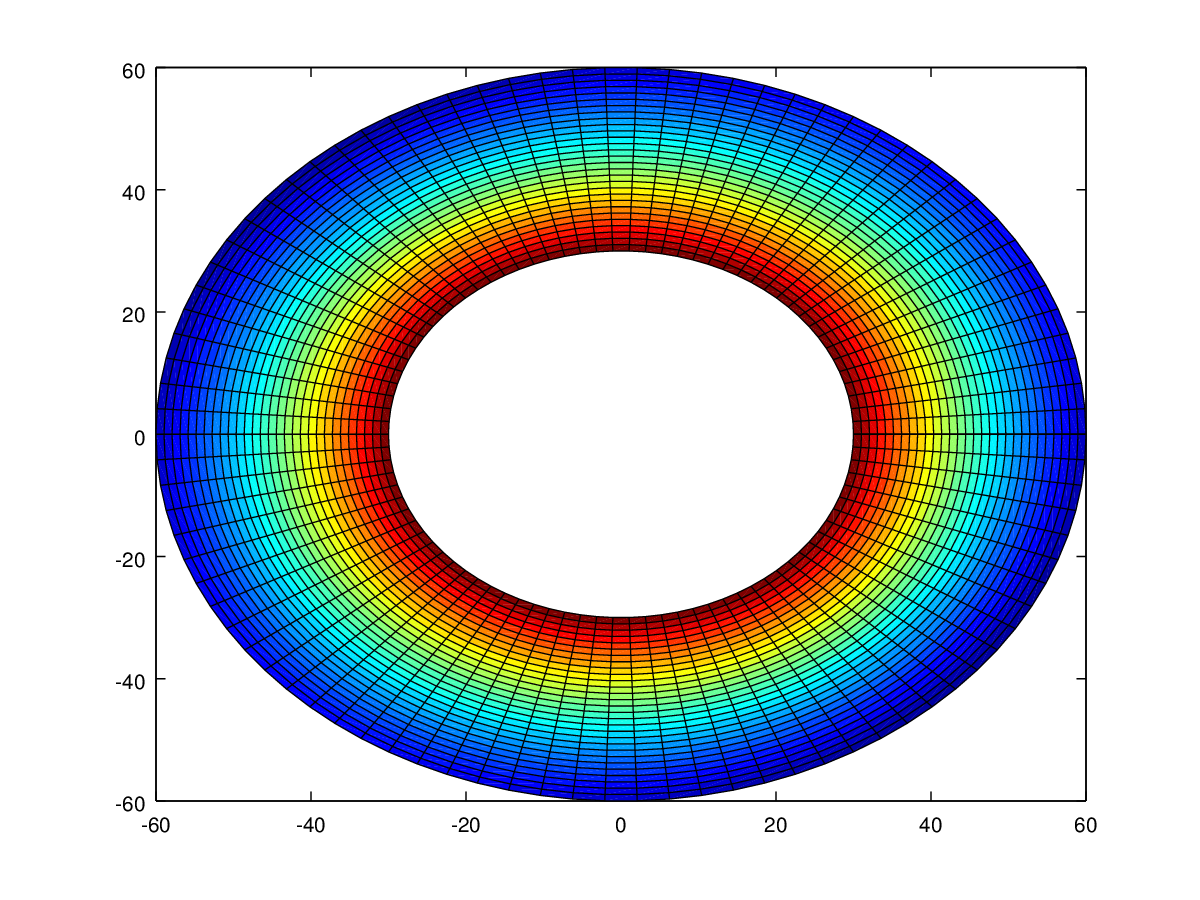
\includegraphics[width=4.5cm]{graficos/1/1b-30.png} \\
      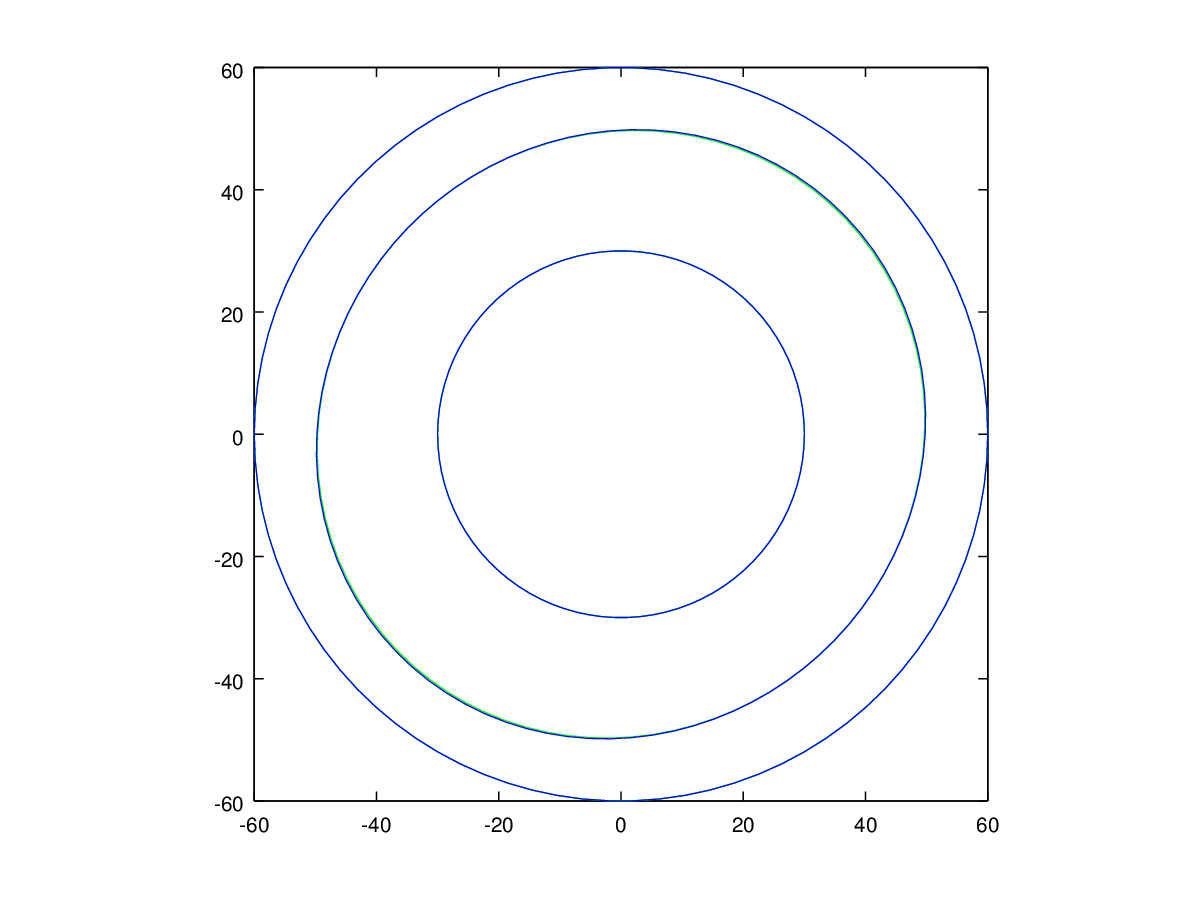
\includegraphics[width=4.5cm]{graficos/1/1b-3-iso.png} &
      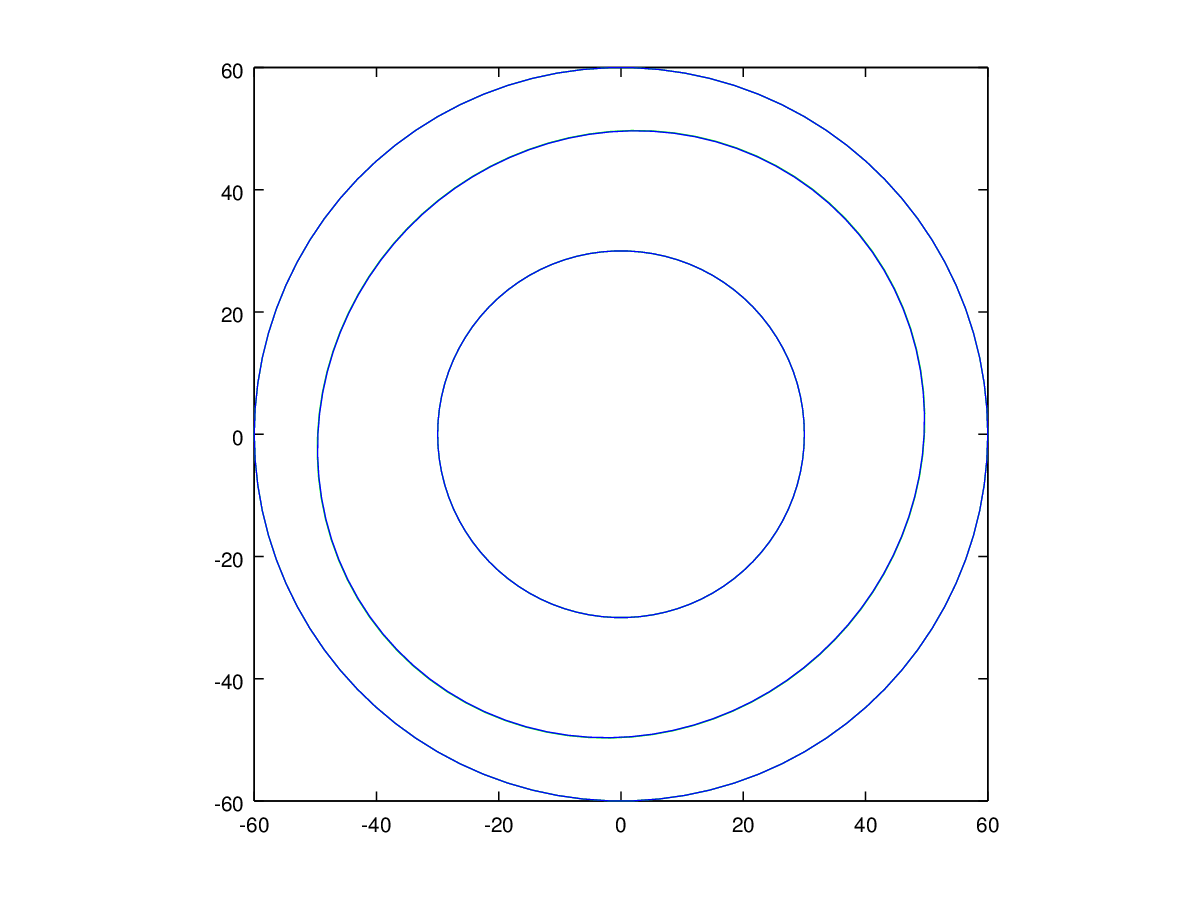
\includegraphics[width=4.5cm]{graficos/1/1b-8-iso.png} &
      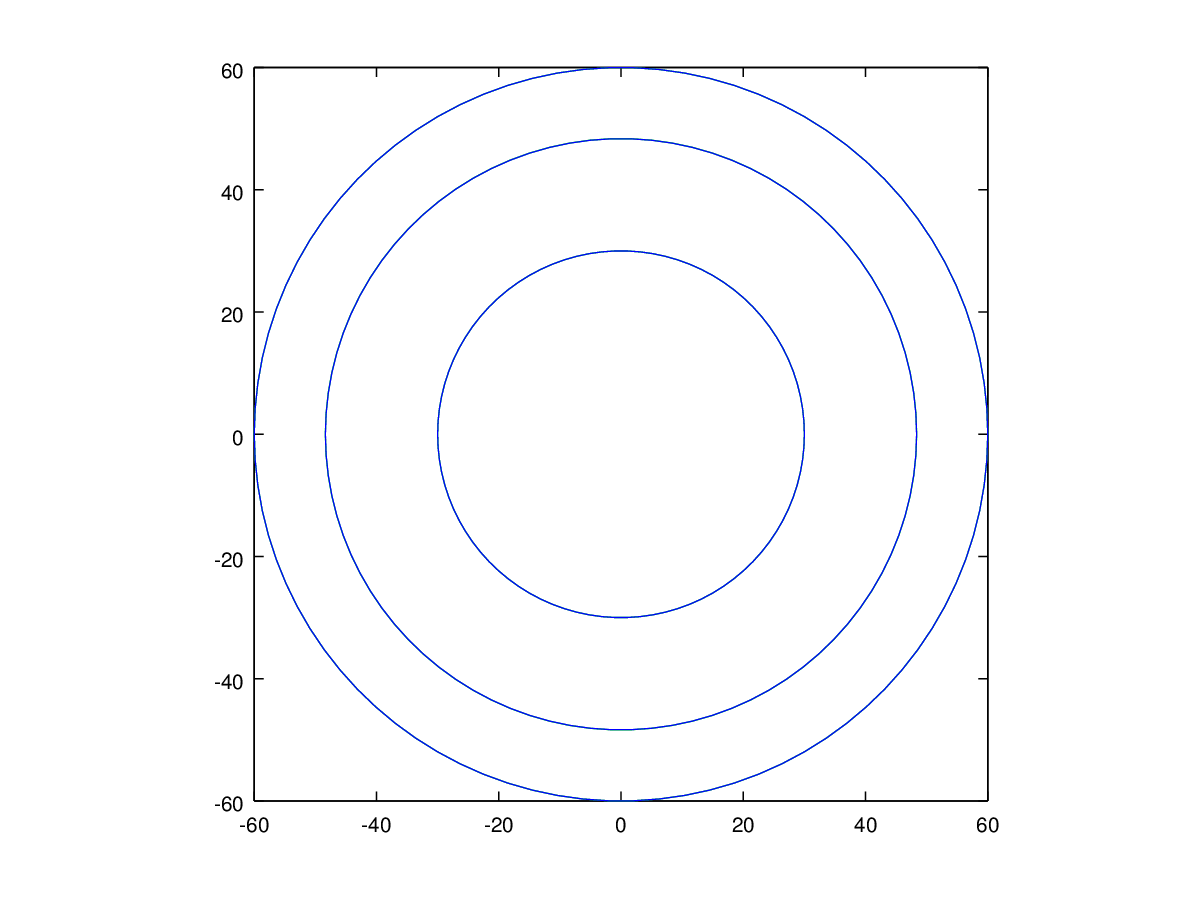
\includegraphics[width=4.5cm]{graficos/1/1b-30-iso.png} \\
      {\small $m+1 = 3$} &
      {\small $m+1 = 8$} &
      {\small $m+1 = 30$} \\
    \end{tabular}}

  \subsubsection*{Experimento 2: Posición de la isoterma según granularidad}

    Para ambos casos se consideraron instancias de prueba con los siguientes parámetros: $r_i = 30$, $r_e = 60$, $T_i = 1500$, $iso = 500$. Se generó una instancia de prueba con una temperatura externa variable entre 50 y 200{\degree}C\footnote{Para la generación de las instancias de prueba se consideró la función $T_e(\theta) = 125 + 75 \sin(2\theta)$} en todos los puntos $(r_e, \theta)$ de la discretización.

    En primer lugar, se calculó la solución del sistema y la posición estimada de la isoterma para una discretización considerablemente granular, con $m + 1 = 70$ y $n = 90$, para utilizar como caso de contraste. Reproducimos los gráficos que representan las temperaturas calculadas para todos los puntos de la discretización y la ubicación estimada de la isoterma.

    {\centering \begin{tabular}{cc}
      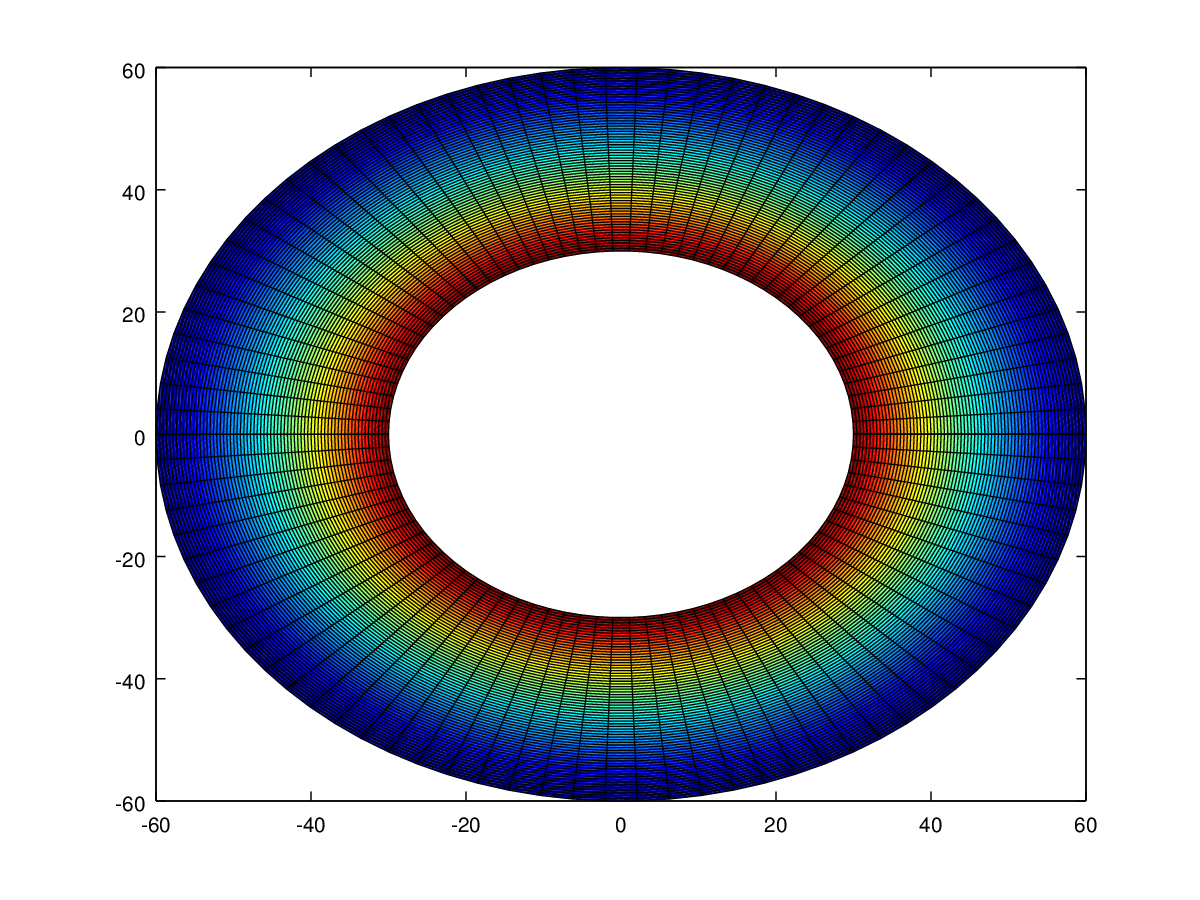
\includegraphics[height=5cm]{graficos/2/2-real.png} & 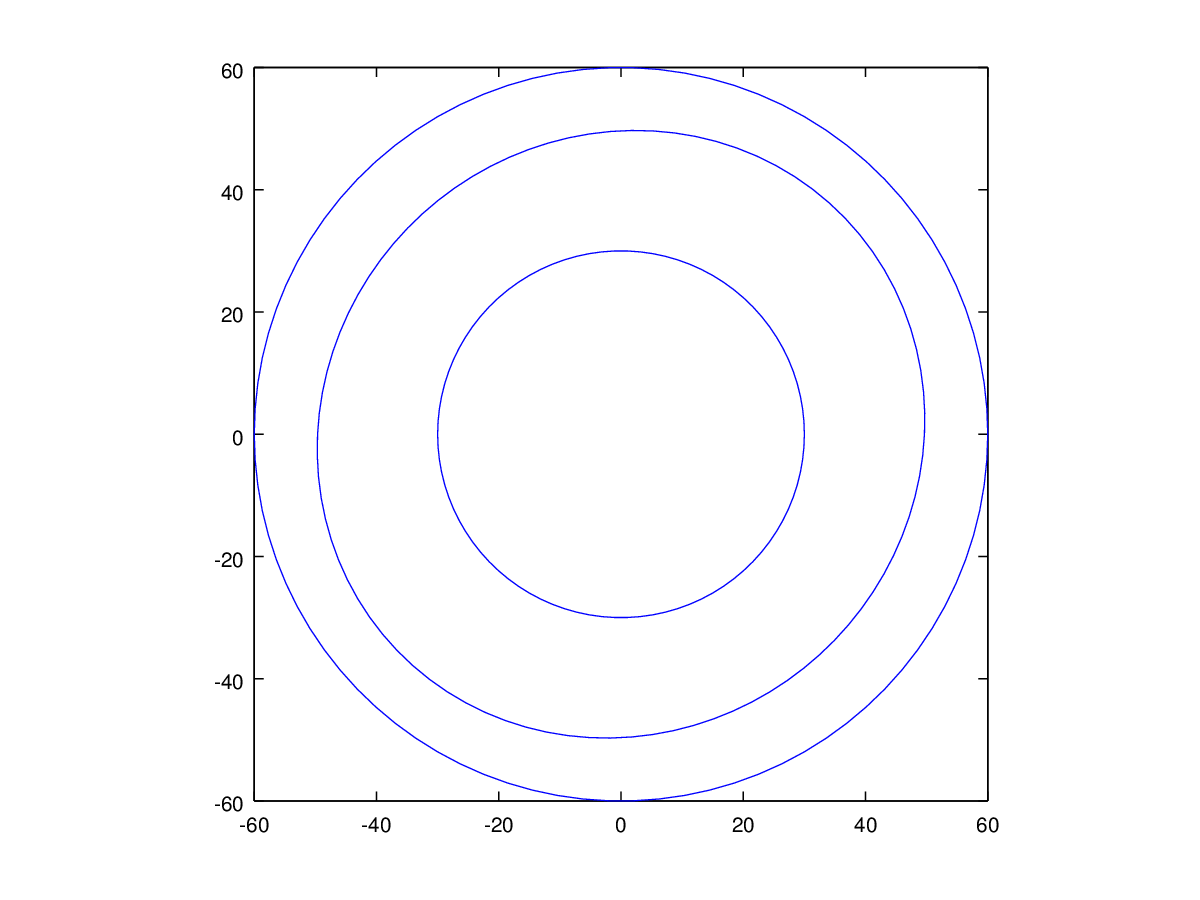
\includegraphics[height=5cm]{graficos/2/2-real-iso.png} \\
      {\small Temperaturas obtenidas} &
      {\small Posición estimada de la isoterma 500{\degree}C} \\
    \end{tabular}}

    \paragraph{Caso A} Se mantuvo constante la cantidad de radios de la discretización $m + 1 = 70$, y se tomaron instancias con diferentes cantidades de ángulos, para $n = 3, 5, 8, 10, 30, 50, 70$. Los gráficos que incluimos representan los resultados obtenidos para $n = 5, 10, 50$, reflejando las temperaturas calculadas y la ubicación estimada de la isoterma (en azul), comparada con la obtenida para el caso de contraste (en verde).

    {\centering \begin{tabular}{ccc}
      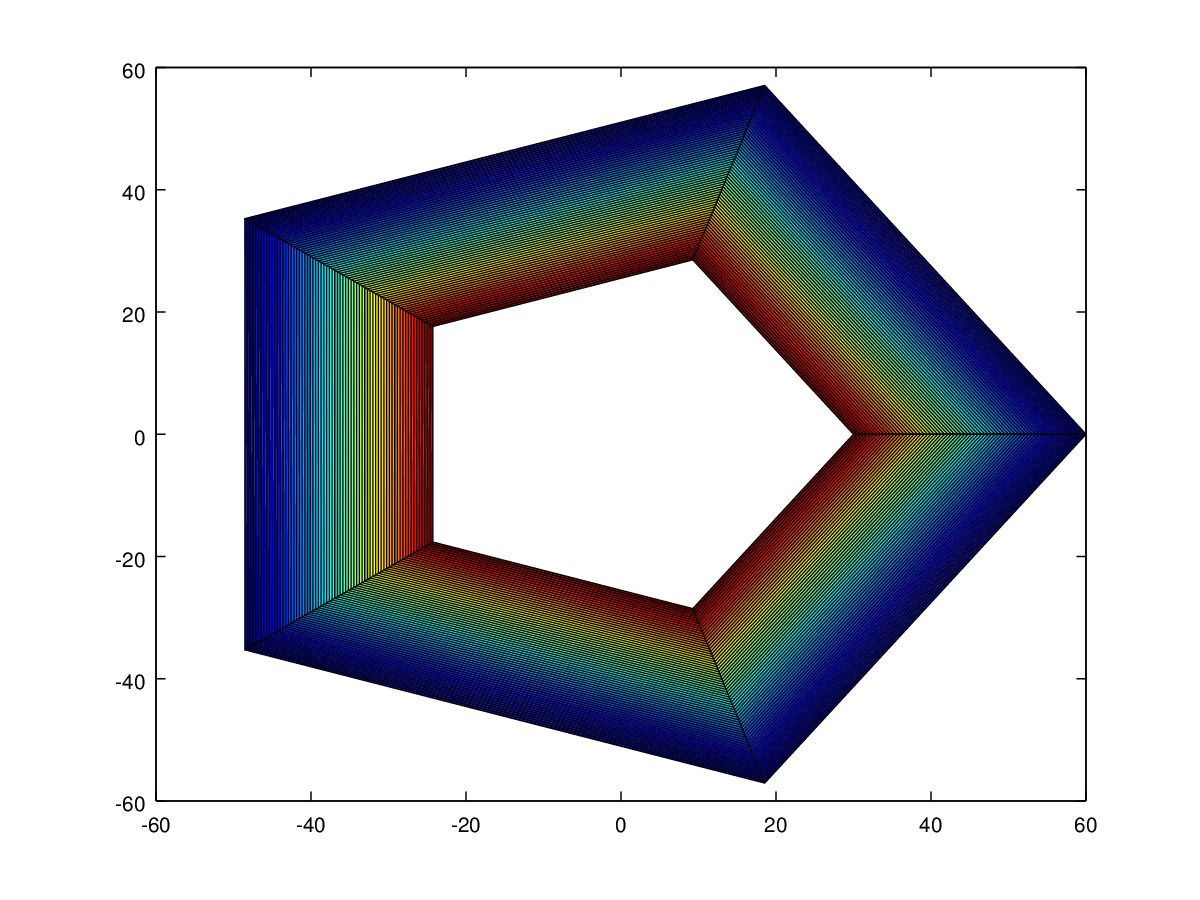
\includegraphics[width=4.5cm]{graficos/2/2a-5.png} &
      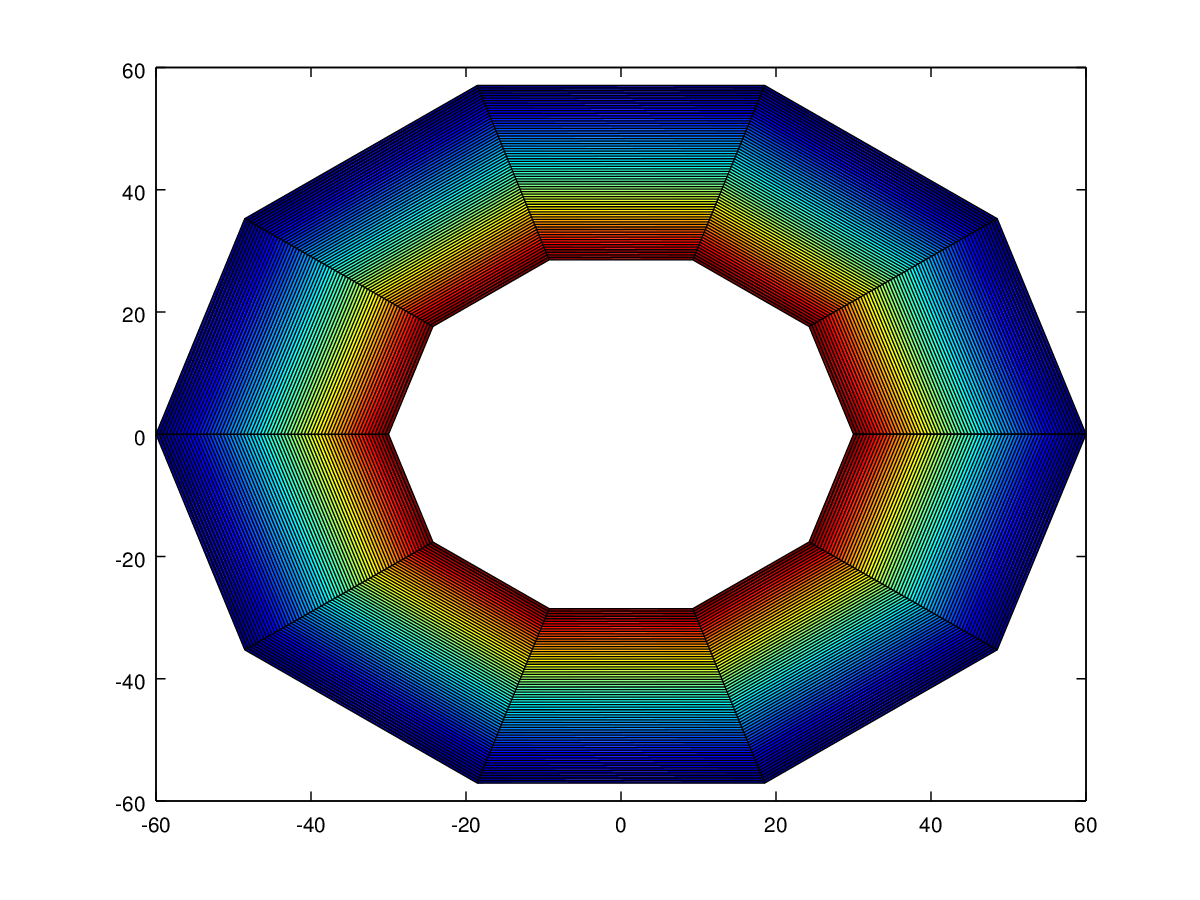
\includegraphics[width=4.5cm]{graficos/2/2a-10.png} &
      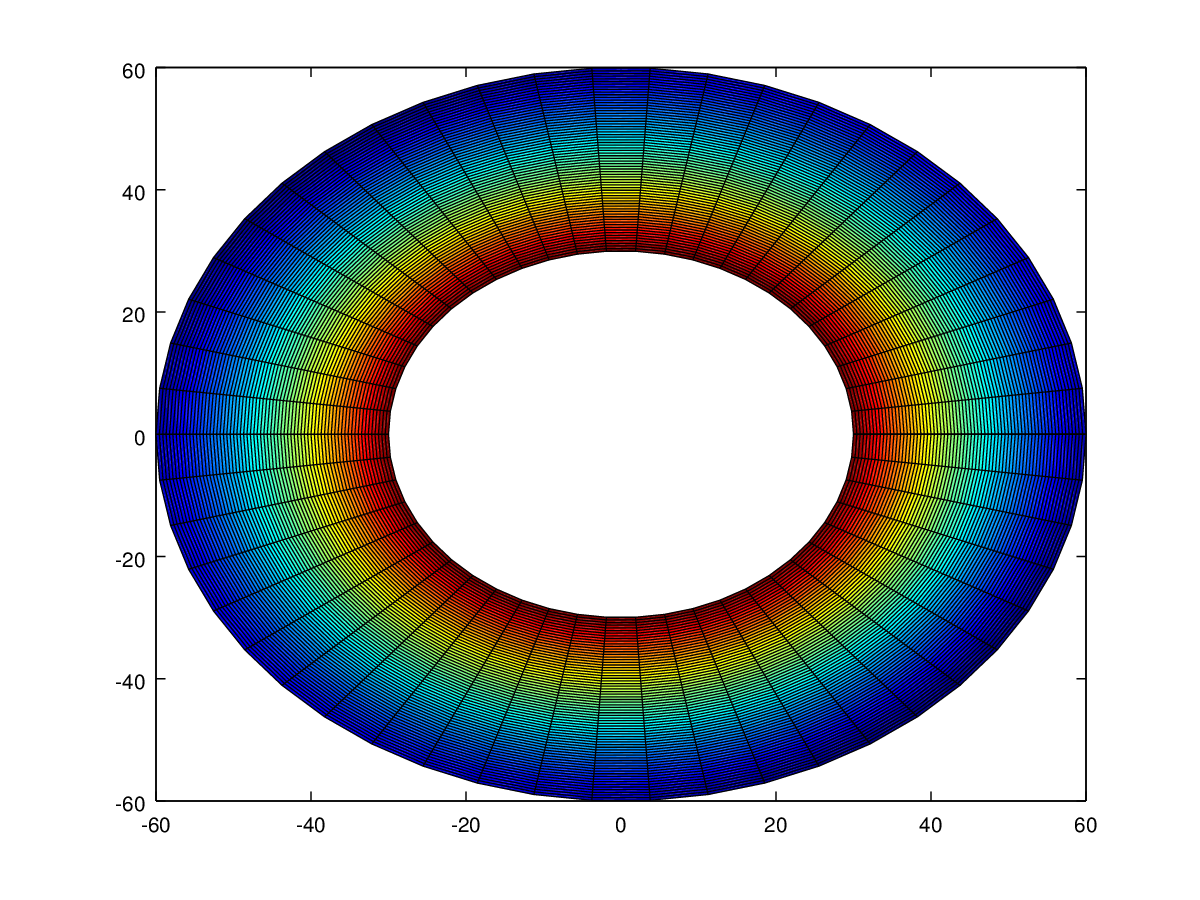
\includegraphics[width=4.5cm]{graficos/2/2a-50.png} \\
      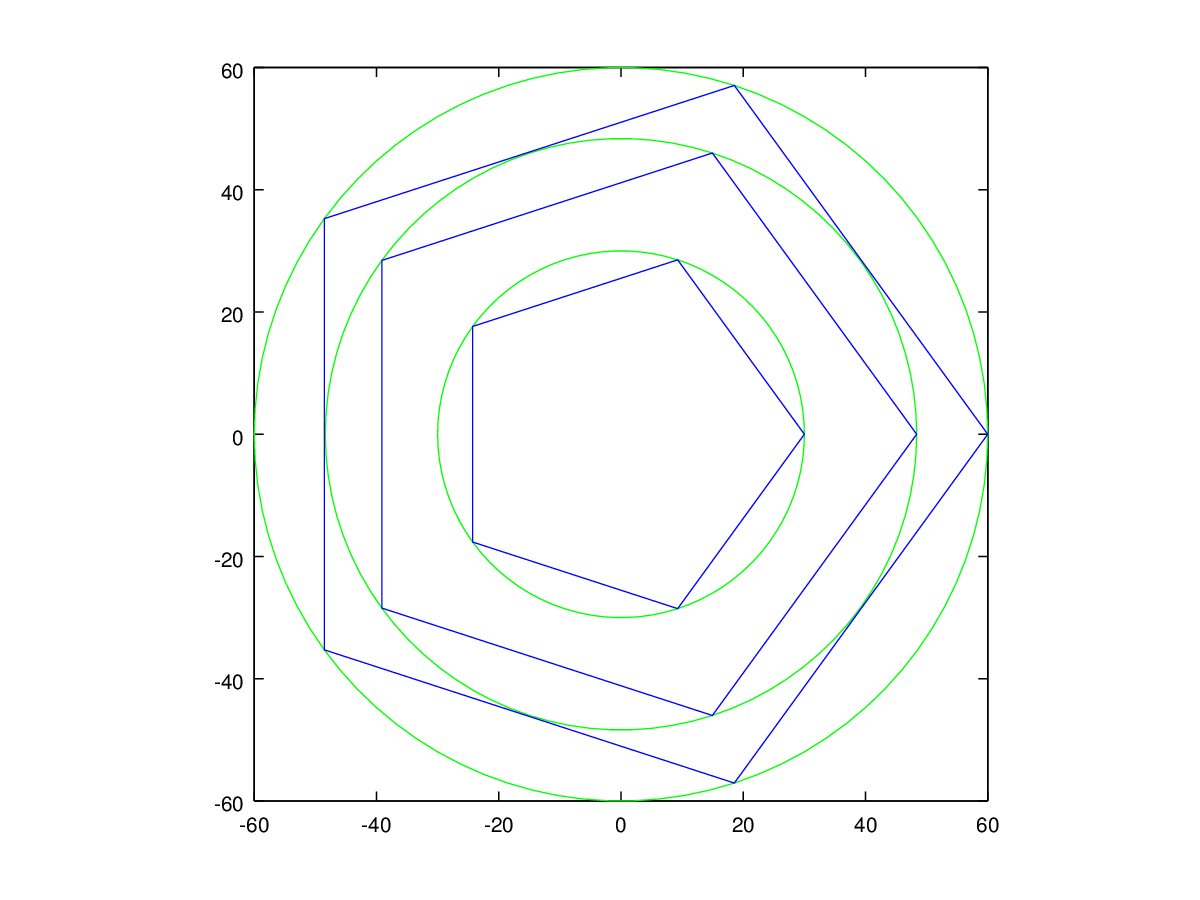
\includegraphics[width=4.5cm]{graficos/2/2a-5-iso.png} &
      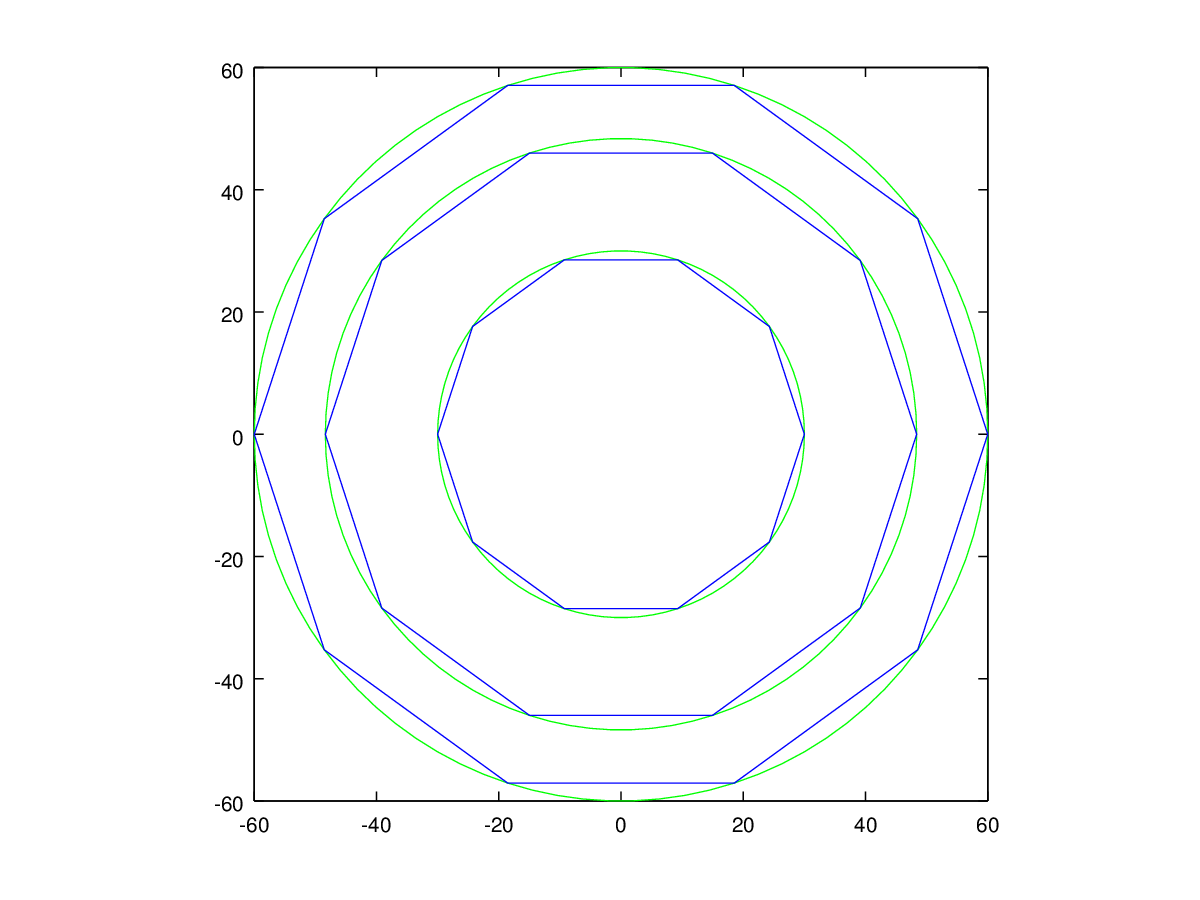
\includegraphics[width=4.5cm]{graficos/2/2a-10-iso.png} &
      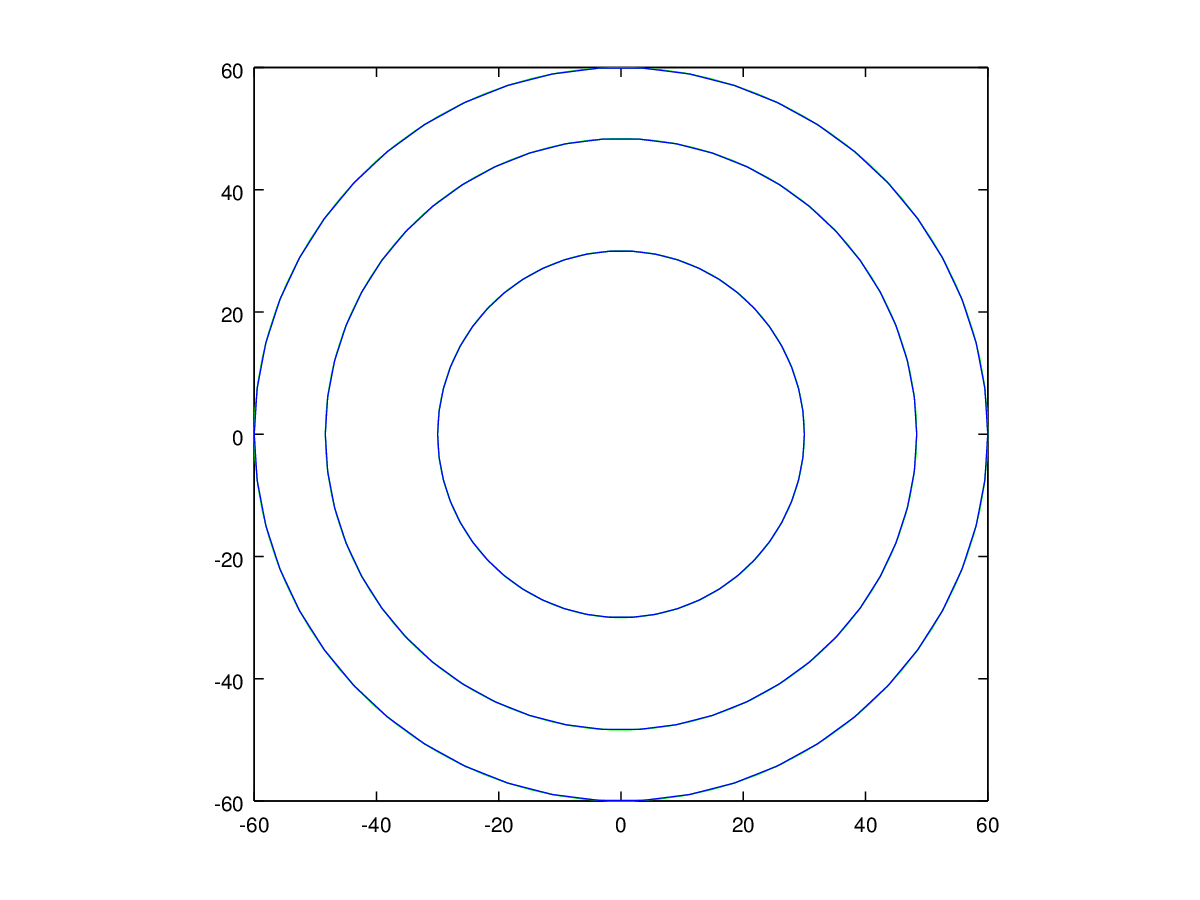
\includegraphics[width=4.5cm]{graficos/2/2a-50-iso.png} \\
      {\small $n = 5$} &
      {\small $n = 10$} &
      {\small $n = 50$} \\
    \end{tabular}}

    \paragraph{Caso B} Se mantuvo constante la cantidad de ángulos de la discretización $n = 90$, y se tomaron instancias con diferentes cantidades de ángulos, para $m + 1 = 3, 5, 8, 10, 30, 50$. Los gráficos que incluimos representan los resultados obtenidos para $m + 1 = 3, 8, 30$, reflejando las temperaturas calculadas y la ubicación estimada de la isoterma (en azul), comparada con la obtenida para el caso de contraste (en verde).

    {\centering \begin{tabular}{ccc}
      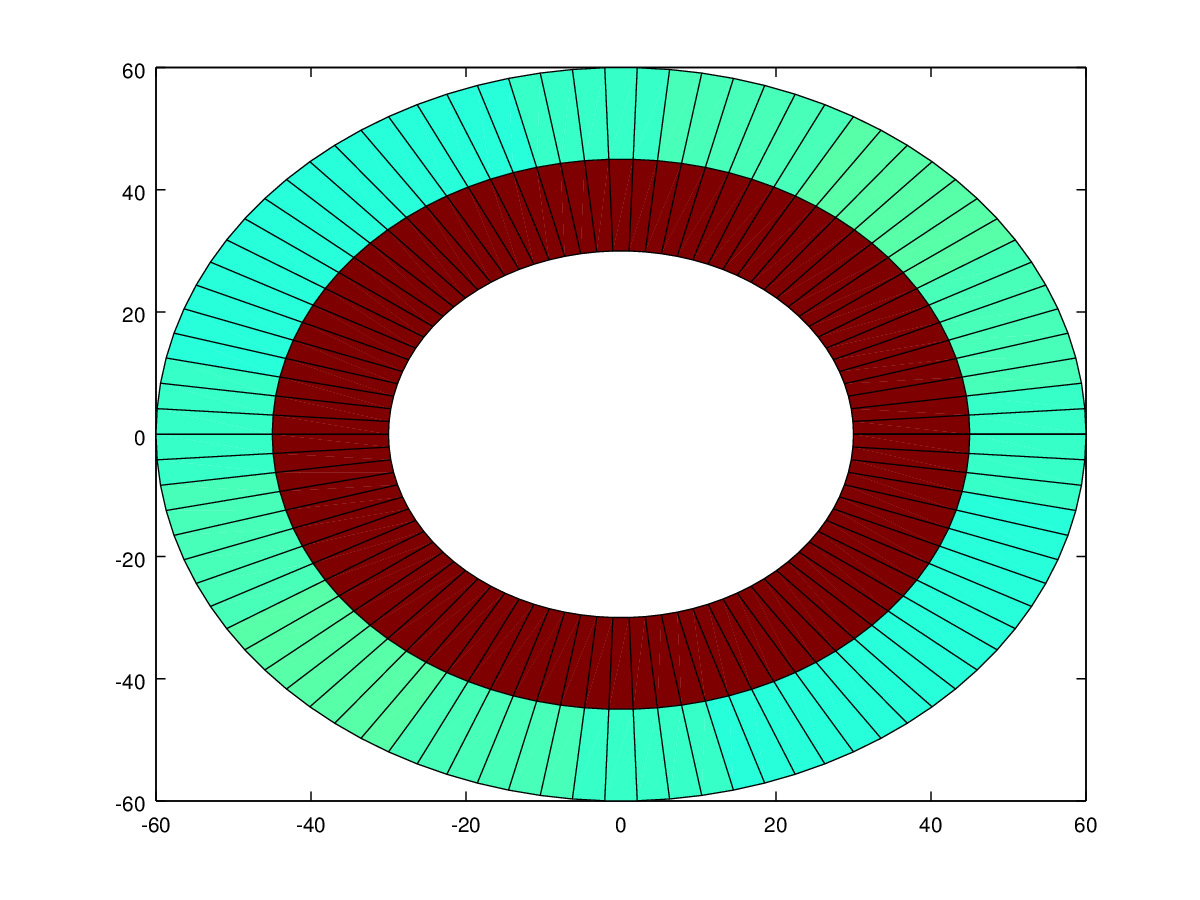
\includegraphics[width=4.5cm]{graficos/1/1b-3.png} &
      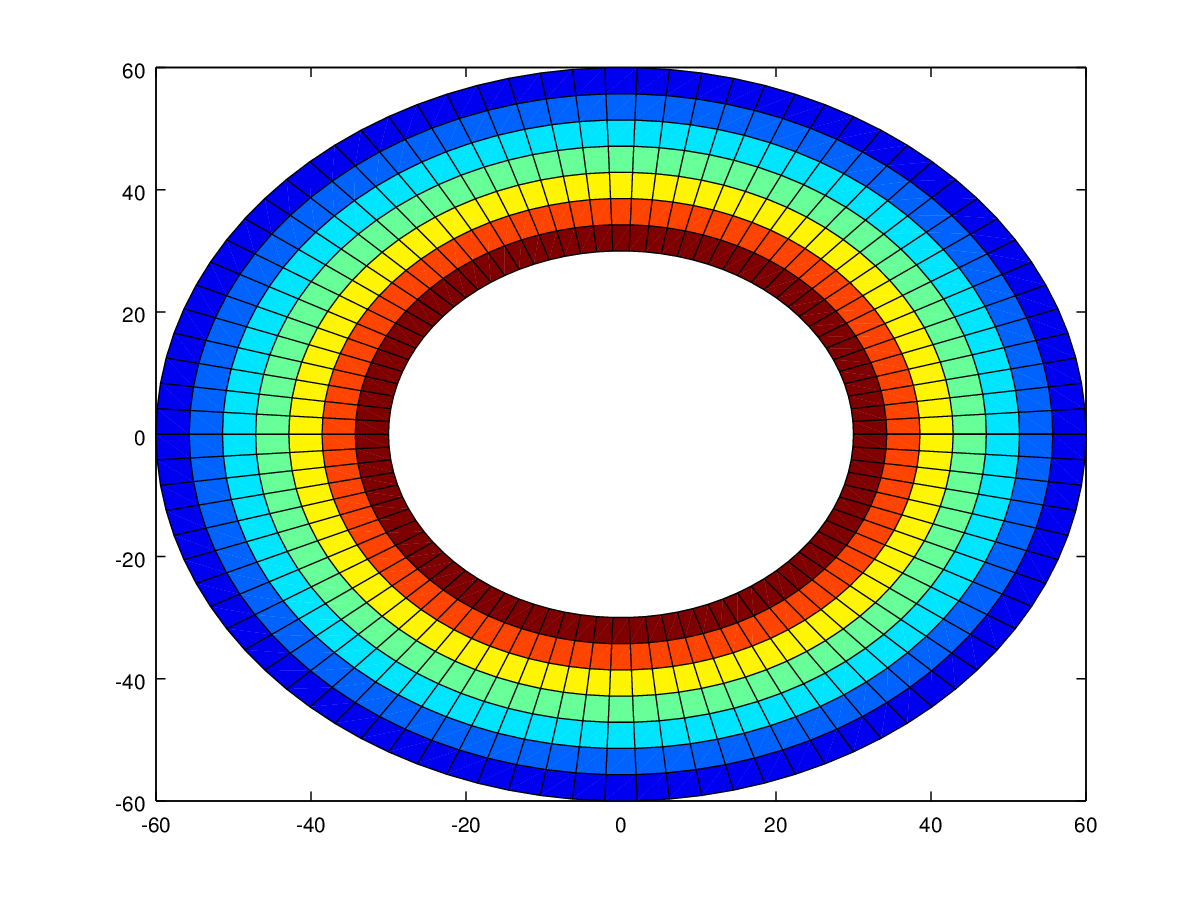
\includegraphics[width=4.5cm]{graficos/1/1b-8.png} &
      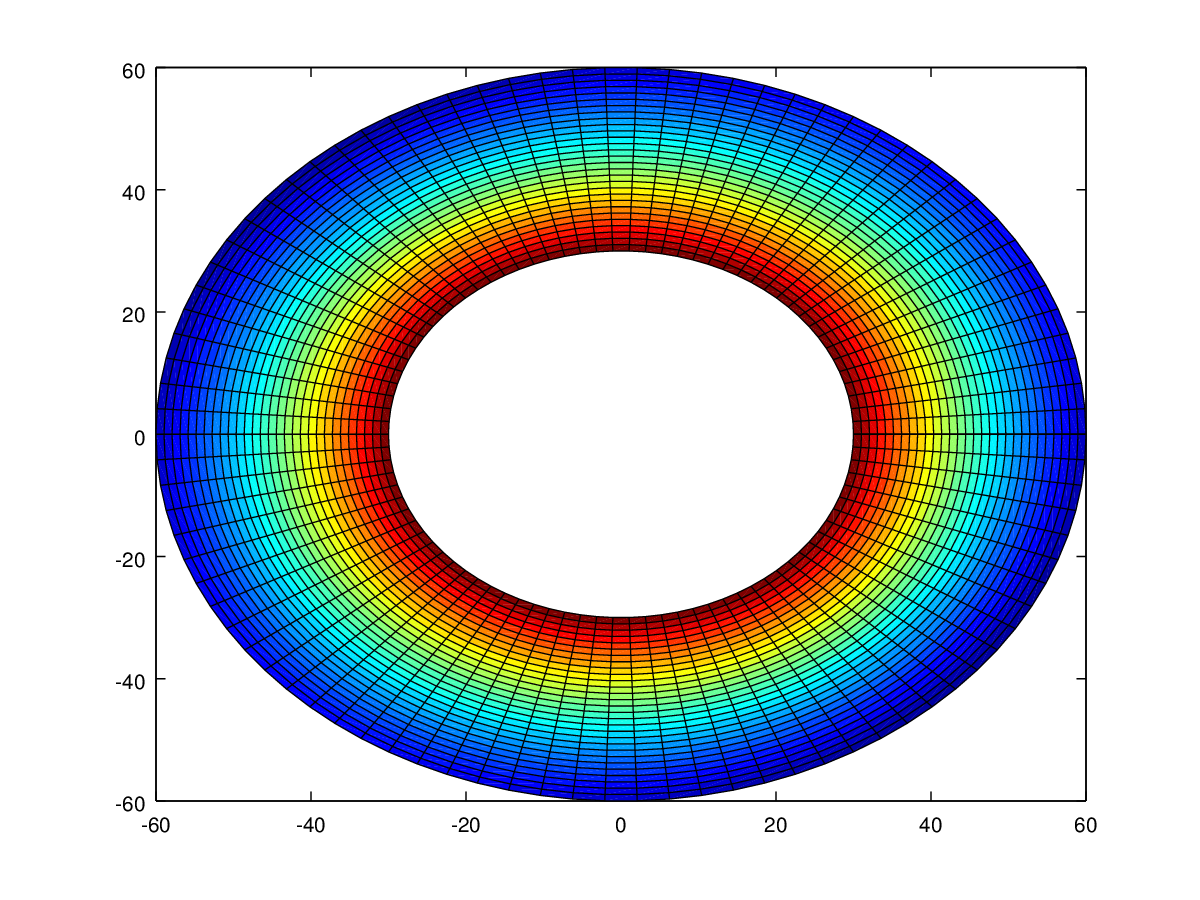
\includegraphics[width=4.5cm]{graficos/1/1b-30.png} \\
      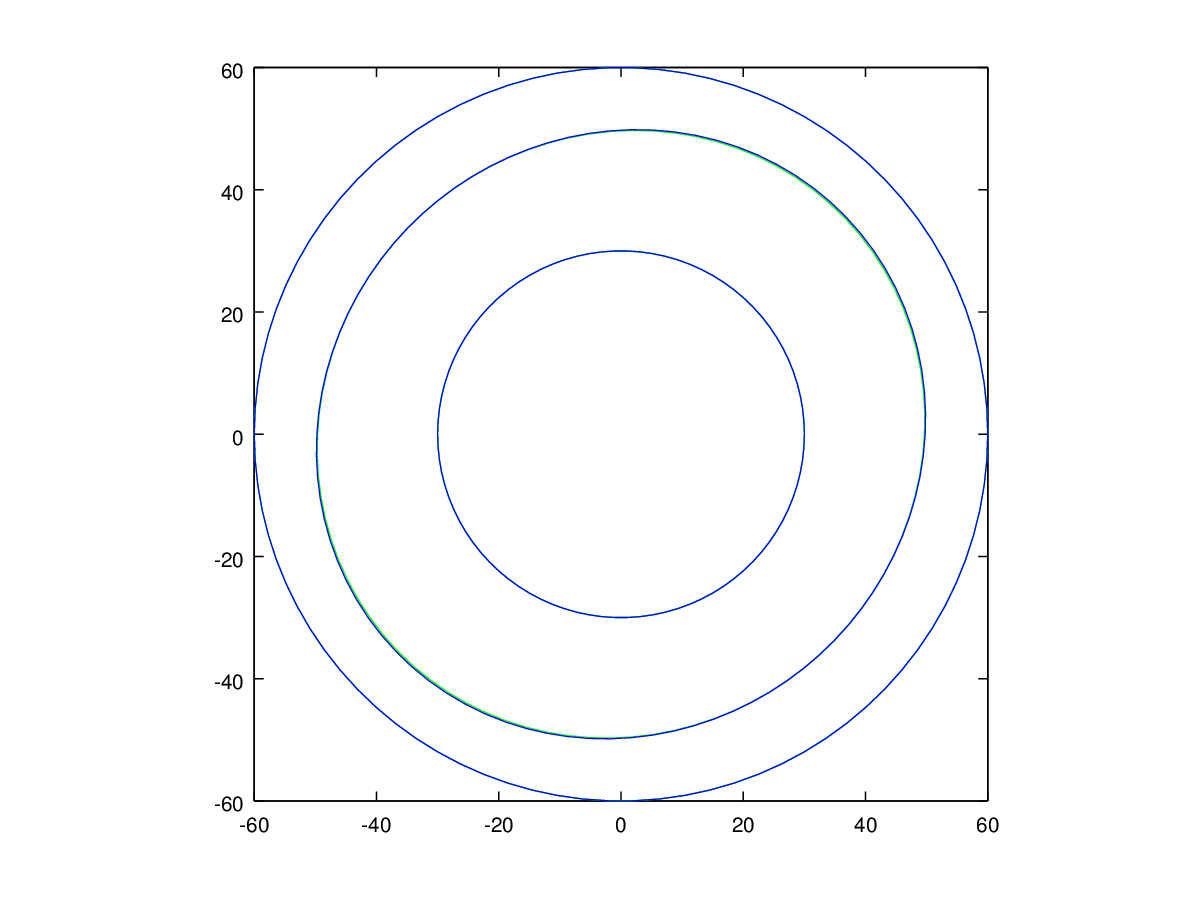
\includegraphics[width=4.5cm]{graficos/1/1b-3-iso.png} &
      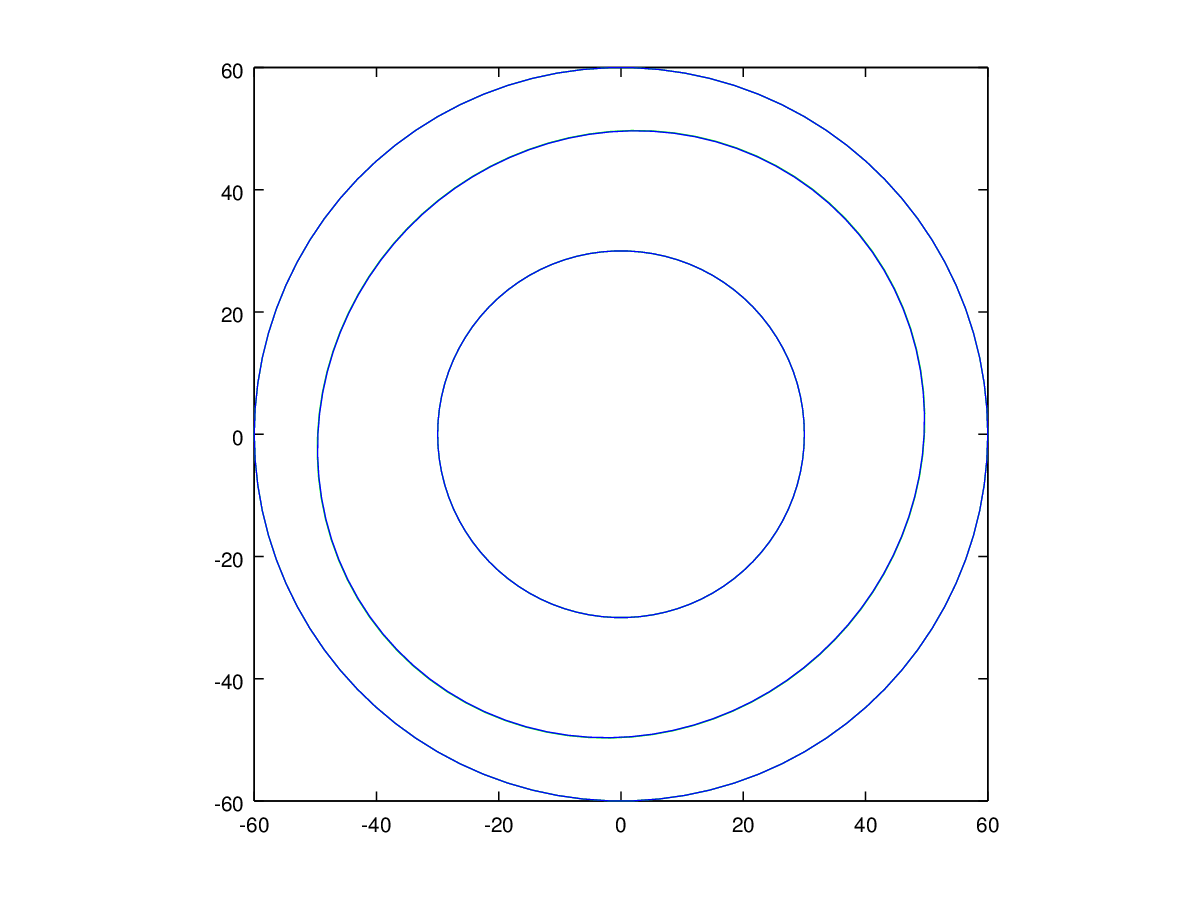
\includegraphics[width=4.5cm]{graficos/1/1b-8-iso.png} &
      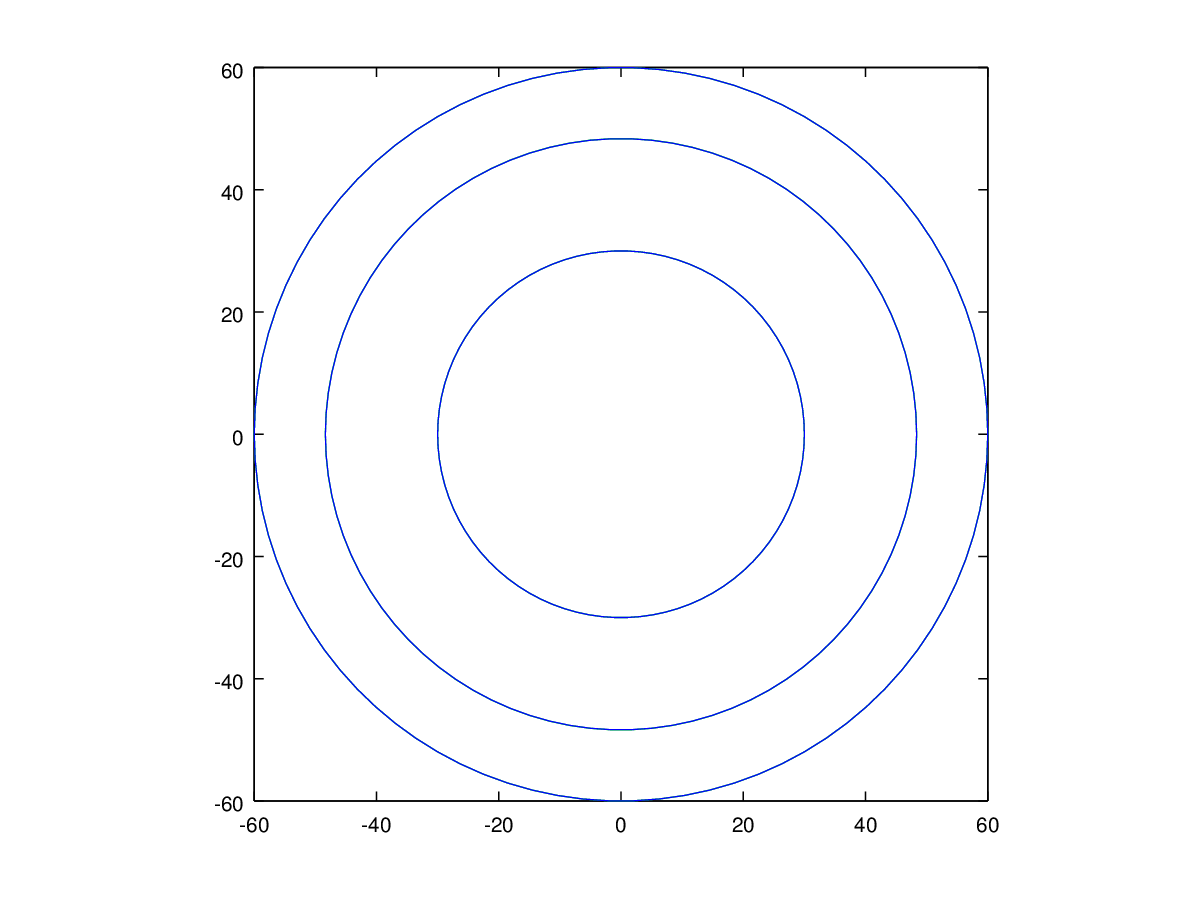
\includegraphics[width=4.5cm]{graficos/1/1b-30-iso.png} \\
      {\small $m+1 = 3$} &
      {\small $m+1 = 8$} &
      {\small $m+1 = 30$} \\
    \end{tabular}}

  \subsubsection*{Experimento 3: Posición de la isoterma según condiciones de borde}

    Se evaluaron dos escenarios de prueba, ambos con los siguientes parámetros: $r_i = 30$, $r_e = 60$, $m+1 = 30$, $n = 30$, $T_i = 1500$, $iso = 500$. Se utilizaron temperaturas externas constantes en todos los puntos $(r_e, \theta)$ de la discretización, con $T_e(\theta) = 50$ en uno de los casos y $T_e(\theta) = 200$ en el otro.

    En el gráfico puede observarse la ubicación estimada de la isoterma para cada uno de los casos, en rojo para $T_e(\theta) = 50$ y en azul para $T_e(\theta) = 200$.

    \begin{center}
      \includegraphics[width=9cm]{graficos/3/3-iso.png} \\
      {\small Posiciones de las isotermas de 500{\degree}C}
    \end{center}

  \subsubsection*{Experimento 4: Índice de peligrosidad según granularidad}

    Se consideró un escenario con los siguientes parámetros: $r_i = 10$, $r_e = 60$, $T_i = 1500$, $iso = 500$. Para la temperatura externa se tomaron valores arbitrarios entre 50 y 200{\degree}C. Luego, se generaron cinco instancias de prueba con los siguientes pares de valores para $m + 1$ y $n$: $(15, 5), (15, 10), (20, 20), (25, 40), (30, 80)$. Se construyó en primer lugar la instancia de prueba con $n = 80$, y las demás se generaron a partir de esta eliminando los valores de $T_e(\theta_k)$ con $k$ par.

    El experimento arrojó los siguientes resultados:

    \begin{center}
      \begin{tabular}{c|c|c}
        $m+1$ & $n$ & Índice de peligrosidad \\ \hline
         15 & 5 & 0.633849 \\
        15 & 10 & 0.633849 \\
        20 & 20 & 0.635172 \\
        25 & 40 & 0.636719 \\
        30 & 80 & 0.637951
      \end{tabular}
    \end{center}

    En el gráfico pueden observarse los valores obtenidos para el índice de peligrosidad de los cinco casos de prueba, en función de la granularidad de la discretización (considerando como medida de la granularidad el valor $(m+1)n$).

    \begin{center}
      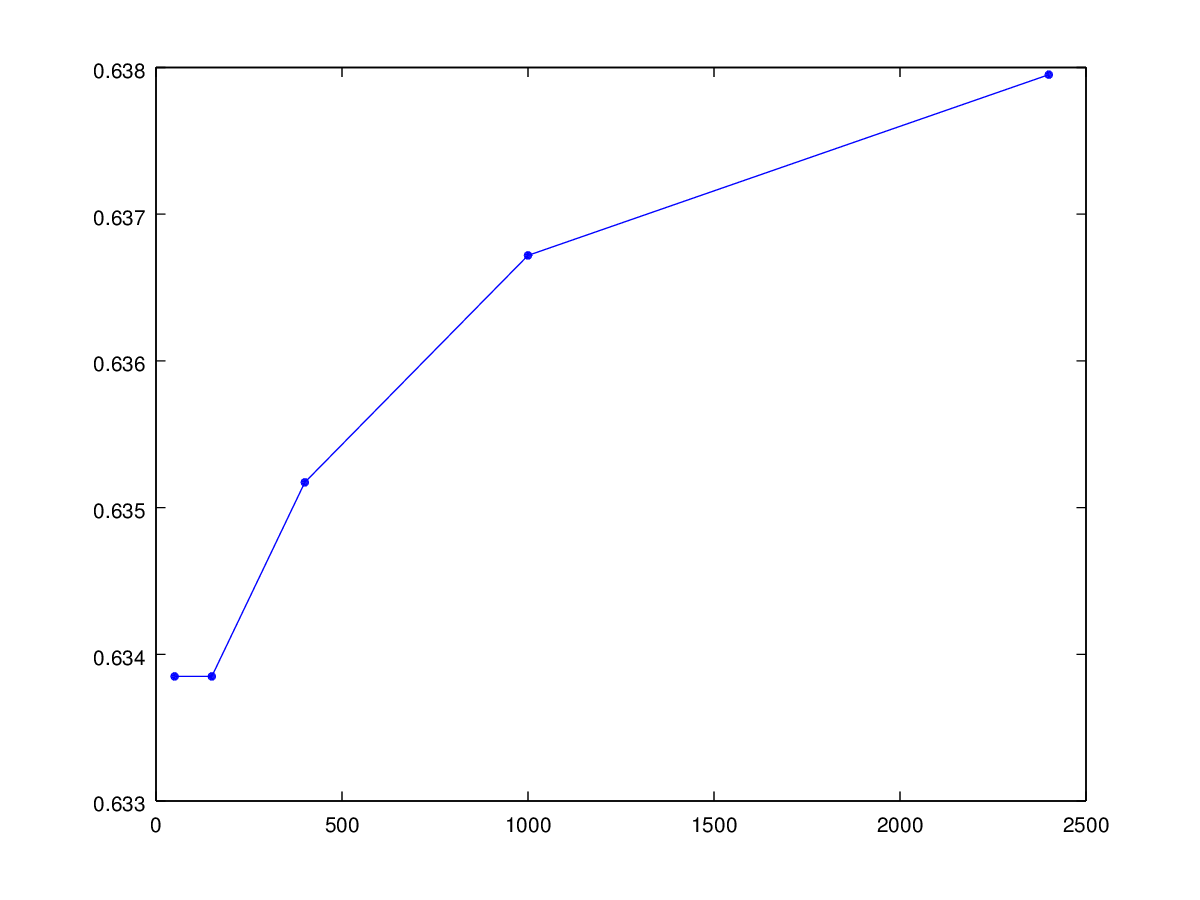
\includegraphics[width=9cm]{graficos/4/4.png} \\
      {\small Índice de peligrosidad en función de la granularidad de la discretización}
    \end{center}

  \subsubsection*{Experimento 5: Índice de peligrosidad según ancho de la pared}

    Para este experimento se mantuvieron constantes los parámetros, $r_e = 90$, $m+1 = 30$, $n = 80$, $T_i = 1500$, $iso = 500$, como así también la temperatura externa $T_e(\theta)$, para la cual se tomaron valores arbitrarios entre 50 y 200{\degree}C. Se generaron instancias con los siguientes valores de $r_i$: $5, 10, 20, 40, 60, 80, 90$. El experimento arrojó los siguientes resultados:

    \begin{center}
      \begin{tabular}{c|c}
        $r_i$ & Índice de peligrosidad \\ \hline
        5 & 0.441240 \\
        10 & 0.557452 \\
        20 & 0.683942 \\
        40 & 0.822686 \\
        60 & 0.909080 \\
        80 & 0.973116 \\
        90 & 1.000000
      \end{tabular}
    \end{center}

    En el gráfico pueden observarse los valores obtenidos para el índice de peligrosidad en función de los diferentes valores de $r_i$.

    \begin{center}
      \includegraphics[width=9cm]{graficos/5/5.png} \\
      {\small Índice de peligrosidad en función del valor de $r_i$}
    \end{center}

  \subsubsection*{Experimento 6: Tiempo de ejecución según número de instancias}

    Se consideró una serie de 6 instancias del problema con los siguientes parámetros: $r_i = 10$, $r_e = 60$, $m+1 = 25$, $n = 40$, $T_i = 1500$, $iso = 500$. Para las temperaturas externas se tomaron valores arbitrarios entre 50 y 200{\degree}C, diferentes en cada una de las instancias.

    Se procesaron sucesivamente 1, 2, 3, 4, 5 y 6 instancias en corridas únicas del programa, utilizando primero el método de Eliminación Gaussiana y luego el de Factorización LU. Los tiempos de ejecución se tomaron en segundos, utilizando la librería \texttt{ctime} de \texttt{C++}. Para las pruebas se omitió realizar la estimación de la posición de la isoterma, limitándose a resolver el sistema por el método elegido. Los valores obtenidos fueron los siguientes:

      \begin{center}
        \begin{tabular}{c|c|c}
          \multirow{2}{*}{$ninst$} & \multicolumn{2}{c}{Tiempo de ejecución(segundos)} \\ 
          & Eliminación Gaussiana & Factorización LU \\ \hline
          1 & 3.099746 & 3.088397 \\
          2 & 6.204906 & 3.089928 \\
          3 & 9.333475 & 3.107586 \\
          4 & 12.392685 & 3.109775 \\
          5 & 15.497981 & 3.119630 \\
          6 & 18.562135 & 3.123978 \\
        \end{tabular}
      \end{center}

    \begin{center}
      \includegraphics[width=9cm]{graficos/6/6.png} \\
      {\small Tiempo de ejecución en función del número de instancias del problema}
    \end{center}

  \subsubsection*{Experimento 7: Tiempo de ejecución según granularidad}

    Para ambos casos, se construyeron escenarios de prueba con los siguientes parámetros: $r_i = 30$, $r_e = 60$, $T_i = 1500$, $iso = 500$. La temperatura externa se consideró constante, con $T_e(\theta) = 50$ para todo $\theta$. En ambos casos las pruebas se realizaron utilizando primero el método de Eliminación Gaussiana y luego el de Factorización LU, y los tiempos de ejecución se tomaron en segundos, utilizando la librería \texttt{ctime} de \texttt{C++}. Para las pruebas se omitió realizar la estimación de la posición de la isoterma, limitándose a resolver el sistema por el método elegido.

    \paragraph{Caso A}
      Se realizaron pruebas variando la cantidad de ángulos de la discretización, con $m + 1 = 30$ y $n = 10, 30, 50, 70, 90$. Los valores obtenidos fueron los siguientes:

      \begin{center}
        \begin{tabular}{c|c|c}
          \multirow{2}{*}{$n$} & \multicolumn{2}{c}{Tiempo de ejecución(segundos)} \\ 
          & Eliminación Gaussiana & Factorización LU \\ \hline
          10 & 0.09335425 & 0.09196125 \\
          30 & 2.25882775 & 2.25695850 \\
          50 & 10.40710775 & 10.40538050 \\
          70 & 28.47581550 & 28.50210100 \\
          90 & 60.43221975 & 60.50333525 \\
        \end{tabular}
      \end{center}

      \begin{center}
        \includegraphics[width=9cm]{graficos/7/7a.png} \\
        {\small Tiempo de ejecución en función de la cantidad de ángulos de la discretización}
      \end{center}

    \paragraph{Caso B}
      Se realizaron pruebas variando la cantidad de radios de la discretización, con $n = 60$ y $m+1 = 10, 30, 50, 70$. Los valores obtenidos fueron los siguientes:

      \begin{center}
        \begin{tabular}{c|c|c}
          \multirow{2}{*}{$m + 1$} & \multicolumn{2}{c}{Tiempo de ejecución(segundos)} \\ 
          & Eliminación Gaussiana & Factorización LU \\ \hline
          10 & 0.67524000 & 0.67400350 \\
          30 & 17.94450675 & 17.98105550 \\
          50 & 82.86414400 & 83.05790825 \\
          70 & 227.07038100 & 227.68770850 \\
        \end{tabular}
      \end{center}

      \begin{center}
        \includegraphics[width=9cm]{graficos/7/7b.png} \\
        {\small Tiempo de ejecución en función de la cantidad de radios de la discretización}
      \end{center}

\clearpage
\section{Discusión}

{
\subsubsection*{Experimento 1: Isoterma según granularidad - constante}
	En este experimento se puede observar que cuando cambiamos los ángulos la isoterma se aleja mucho más de la real que cuando variamos los radios. Esto es asi ya que comparando los errores de dejar de considerar temperaturas y el error de tomar una medida como lineal cuando no lo es, la primera es peor y distorsiona mucho más la isoterma.
	


\subsubsection*{Experimento 2: Isoterma según granularidad -seno}
	En este caso se observa lo mismo que en el anterior ya que lo único que estamos variando es que las temperaturas de la pared externa ahora no son constantes. Ésto no modifica el error de aproximar la isoterma con menos discretizacion en los ángulos o en los radios.



\subsubsection*{Experimento 3: Índice de peligrosidad según granularidad}
  	En el gráfico presentado, se puede notar que no hay diferencia entre los índices de las instancias con 5 y 10 particiones sobre ángulos, ya que al calcularlos utilizando el método explicado anteriormente, el punto más cercano a la pared en la primera, fue considerado en la segunda. 

  	En cambio, en el resto de las instancias, el índice de peligrosidad aumenta, ya que al tomar más particiones, fueron tomados en cuenta nuevos puntos, afectando la isoterma, y por lo tanto, el índice. 

  	De esta forma, demostramos experimentalmente nuestra hipótesis. 


\subsubsection*{Experimento 4}
	En este experimento se puede ver que a medida que disminuimos el grosor de la pared del alto horno la isoterma se encuentra cada vez mas cerca de la pared externa. El índice de peligrosidad mide la relación entre la temperatura más alta y la proximidad de la misma a la pared externa. 

	Cuando disminuimos el grosor de la pared, lo que hacemos es acercar la pared interna(donde se encuentra la temperatura más alta del sistema) a la pared externa. De esta forma la isoterma va a estar mas proxima a la pared externa que cuando el grosor es mayor. Entonces el índice de peligrosidad aumentará, demostrando así lo que se planteó en la hipotesis.
	

\subsubsection*{Experimento 5: Tiempo según número de instancias}
	Se observa que cuando hay pocas instancias, buscar la isoterma con el método de eliminacion gaussiana o el de factriazacion LU es muy similar.

	A medida que aumentan las instancias las diferencias entre ambos métodos aumentan, ya que la factorizacion LU se mantiene casi inmutable al aumentar las instancias mientras que la eliminacion gaussiana aumenta notoriamente.

	Se puede observar que lo que tarda la eliminación gaussiana cuando tiene 2 instancias es aproximadamente el doble de lo que tarda cuando es una única instancia. Cuando son 3 instancias, tarda el triple de lo que tarda cuando es una única instancia. 

	Sean n instancias entonces lo que tarda la eliminación gaussiana es lo que tarda cuando es una única instancia n veces. Esto es asi ya que en este método numérico, para cada una de las instancias recalcula toda la matriz. En cambio la factorizacion LU, calcula la matriz una única vez.


\subsubsection*{Experimento 6: Tiempo según granularidad}
  	En los dos gráficos correspondientes a este experimento, es claro el crecimiento del tiempo de ejecución, a medida que la granularidad aumenta, tanto en los ángulos como en los radios. Esto se debe a la complejidad de los algoritmos utilizados.

  	También, es importante notar como el tiempo de ejecución sobre una sola instancia no cambia demasiado al modificar el método de resolución. Sabemos que, cuando se trata de un solo caso, factorización LU tiene complejidad mayor por constantes que eliminación gaussiana, lo que se puede visualizar en los casos con mayor granularidad de la discretización.


\subsubsection*{Experimento 7: relacion de la isoterma con los bordes}
 	En este experimento se puede ver que la isoterma roja se encuentra mas próxima a la pared interna del horno ya que corresponde a la intancia que tiene menor temperatura en la pared externa (50 grados). Lo mismo ocurre con la isoterma azúl que se encuentra mas cerca de la pared externa debido a que las temperaturas son mas altas (200 grados).

 	Ademas, en uno de los casos la tempreartura externa es la máxima posible y en el otro la mínima. Podemos observar que nunca, con esta discretización, para ningún valor de temperaturas externas válidas, la isoterma puede pasar mas cerca de la pared externa del alto horno que lo que pasa la isoterma marcada en el grafico con azul. Tampoco tampoco es posible que la isoterma pase mas cerca de la pared interna del horno de lo que pasa la isoterma marcada en el grafico con color rojo.
}

\clearpage
\section{Conclusiones}

  La primer gran conclusión que pudimos sacar fue que el método numérico de factorización LU es mucho más eficiente que el de eliminación gausseana cuando tenemos varias instancias. Para una cantidad chica de instancias son muy similares entre si. Ésto lo pudimos observar mediante los experimentos en los cuales comparabamos los tiempos de ejecución entre ambos métodos para valores de entrada con diferentes cantidades de instancias. 

  Otra de las conclusiones fue que cuanto mayor sea la granularidad, la isoterma se aproxima más al valor real. También concluimos que disminuir la cantidad de particiones de ángulos hace que la isoterma se aleje más de la real que disminuir las de los radios. Esto lo vimos tomando como real una isoterma en un sistema muy granularizado, luego disminuimos la granularidad en radios y comparamos entre las isotermas. Después repetimos el experimento pero disminuyendo la cantidad de ángulos.

  Finalmente podemos concluir que para lograr una mayor eficiencia en el cálculo de la isoterma debemos utilizar el método de factorizacion LU y utilizar la mayor cantidad posible de particiones.

\clearpage

% Apéndices
\begin{appendices}

  \section{Enunciado del trabajo práctico}

    \subsection{Introducción}

      Consideremos la sección horizontal de un horno de acero cilíndrico, como en la Figura \ref{fig:seccionHorno}. El sector A es la pared del horno, y el sector B es el horno propiamente dicho, en el cual se funde el acero a temperaturas elevadas. Tanto el borde externo como el borde interno de la pared forman círculos. Suponemos que la temperatura del acero dentro del horno (o sea, dentro de B) es constante e igual a 1500{\degree}C.
      Tenemos sensores ubicados en la parte externa del horno para medir la temperatura de la pared externa del mismo, que habitualmente se encuentra entre 50{\degree}C y 200{\degree}C. El problema que debemos resolver consiste en estimar la isoterma de 500{\degree}C dentro de la pared del horno, para estimar la resistencia de la misma. Si esta isoterma está demasiado cerca de la pared externa del horno, existe peligro de que la estructura externa de la pared colapse.

      \begin{figure}[h]
        \centering
        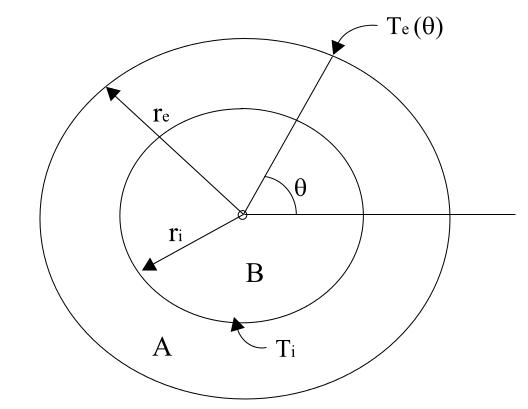
\includegraphics[width=10cm]{seccionHorno.jpg}
        \caption{Sección circular del horno.}
        \label{fig:seccionHorno}
      \end{figure}

      El objetivo del trabajo práctico es implementar un programa que calcule la isoterma solicitada, conociendo las dimensiones del horno y las mediciones de temperatura en la pared exterior.

    \subsection{El Modelo}

      Sea $r_e \in \mathbb{R}$ el radio exterior de la pared y sea $r_i \in \mathbb{R}$ el radio interior de la pared. Llamemos $T(r, \theta)$ a la temperatura en el punto dado por las coordenadas polares $(r, \theta)$, siendo $r$ el radio y $\theta$ el ángulo polar de dicho punto. En el estado estacionario, esta temperatura satisface la ecuación del calor:

      \begin{equation} \label{eq:en1}
        \frac{\partial^2 T(r, \theta)}{\partial r^2} + \frac{1}{r} \frac{\partial T(r, \theta)}{\partial r} + \frac{1}{r^2} \frac{\partial^2 T(r, \theta)}{\partial \theta^2} = 0
      \end{equation}

      Si llamamos $T_i \in \mathbb{R}$ a la temperatura en el interior del horno (sector B) y $T_e : [0, 2\pi] \to \mathbb{R}$ a la función de temperatura en el borde exterior del horno (de modo tal que el punto $(r_e, \theta)$ tiene temperatura $T_e(\theta)$), entonces tenemos que

      \begin{equation} \label{eq:en2}
        T(r, \theta) = T_i \text{ para todo punto } (r, \theta) \text{ con } r \leq r_i
      \end{equation}

      \begin{equation} \label{eq:en3}
        T(r_e, \theta) = T_e(\theta) \text{ para todo punto } (r_e, \theta)
      \end{equation}

      El problema en derivadas parciales dado por la primera ecuación con las condiciones de contorno presentadas recientemente, permite encontrar la función $T$ de temperatura en el interior del horno (sector A), en función de los datos mencionados en esta sección.

      Para resolver este problema computacionalmente, discretizamos el dominio del problema (el sector A) en coordenadas polares. Consideramos una partición $0 = \theta_0 < \theta_1 < ... < \theta_n = 2\pi$ en $n$ ángulos discretos con $\theta_k - \theta_{k-1} = \Delta \theta$ para $k = 1, \dots n$, y una partición $r_i = r_0 < r_1 < ... < r_m = r_e$ en $m + 1$ radios discretos con $r_j - r_{j-1} = \Delta r$ para $j = 1, \dots m$.

      El problema ahora consiste en determinar el valor de la función $T$ en los puntos de la discretización $(r_j, \theta_k)$ que se encuentren dentro del sector A. Llamemos $t_{jk} = T(r_j , \theta_k)$ al valor (desconocido) de la función $T$ en el punto $(r_j, \theta_k)$.

      Para encontrar estos valores, transformamos la ecuación (\ref{eq:en1}) en un conjunto de ecuaciones lineales sobre las incógnitas $t_{jk}$, evaluando (\ref{eq:en1}) en todos los puntos de la discretización que se encuentren dentro del sector A. Al hacer esta evaluación, aproximamos las derivadas parciales de $T$ en (\ref{eq:en1}) por medio de las siguientes fórmulas de diferencias finitas:

      \begin{equation} \label{eq:en4}
        \frac{\partial^2 T(r, \theta)}{\partial r^2}(r_j, \theta_k) \cong \frac{t_{j-1,k} - 2 t_{jk} + t_{j+1,k}}{(\Delta r)^2}
      \end{equation}

      \begin{equation} \label{eq:en5}
        \frac{\partial T(r, \theta)}{\partial r}(r_j, \theta_k) \cong \frac{t_{j,k} - t_{j-1,k}}{\Delta r}
      \end{equation}

      \begin{equation} \label{eq:en6}
        \frac{\partial^2 T(r, \theta)}{\partial \theta^2}(r_j, \theta_k) \cong \frac{t_{j,k-1} - 2 t_{jk} + t_{j,k+1}}{(\Delta \theta)^2}
      \end{equation}

      Es importante notar que los valores de las incógnitas son conocidos para los puntos que se encuentran sobre el borde exterior de la pared, y para los puntos que se encuentren dentro del sector B. Al realizar este procedimiento, obtenemos un sistema de ecuaciones lineales que modela el problema discretizado. La resolución de este sistema permite obtener una aproximación de los valores de la función $T$ en los puntos de la discretización.

    \subsection{Enunciado}
      Se debe implementar un programa en \texttt{C} o \texttt{C++} que tome como entrada los parámetros del problema ($r_i$, $r_e$, $m + 1$, $n$, valor de la isoterma buscada, $T_i$, $T_e(\theta)$) que calcule la temperatura dentro de la pared del horno utilizando el modelo propuesto en la sección anterior y que encuentre la isoterma buscada en función del resultado obtenido del sistema de ecuaciones. El método para determinar la posición de la isoterma queda a libre elección de cada grupo y debe ser explicado en detalle en el informe.

      El programa debe formular el sistema obtenido a partir de las ecuaciones (\ref{eq:en1})-(\ref{eq:en6}) y considerar dos métodos posibles para su resolución: mediante el algoritmo clásico de Eliminación Gaussiana y la Factorización LU. Finalmente, el programa escribirá en un archivo la solución obtenida con el formato especificado en la siguiente sección.

      Como ya se ha visto en la materia, no es posible aplicar los métodos propuestos para la resolución a cualquier sistema de ecuaciones. Sin embargo, la matriz del sistema considerado en el presente trabajo cumple con ser diagonal dominante (no estricto) y que, ordenando las variables y ecuaciones convenientemente, es posible armar un sistema de ecuaciones cuya matriz posee la propiedad de ser \emph{banda}. Luego, se pide demostrar (o al menos dar un esquema de la demostración) el siguiente resultado e incluirlo en el informe:

      \begin{prop}
        Sea $A \in \mathbb{R}^{n \times n}$ la matriz obtenida para el sistema definido por (\ref{eq:en1})-(\ref{eq:en6}). Demostrar que es posible aplicar Eliminación Gaussiana sin pivoteo.\footnote{Sugerencia: Notar que la matriz es diagonal dominante (no estrictamente) y analizar qué sucede al aplicar un paso de Eliminación Gaussiana con los elementos de una fila.}
      \end{prop}

      La solución del sistema de ecuaciones permitirá saber la temperatura en los puntos de la discretización. Sin embargo, nuestro interés es calcular la isoterma 500, para poder determinar si la estructura se encuentra en peligro. Luego, se pide lo siguiente:

      \begin{itemize}
        \item Dada la solución del sistema de ecuaciones, proponer una forma de estimar en cada ángulo de la discretización la posición de la isoterma 500.
        \item En función de la aproximación de la isoterma, proponer una forma (o medida) a utilizar para evaluar la peligrosidad de la estructura en función de la distancia a la pared externa del horno.
      \end{itemize}

      En función de la experimentación, se busca realizar dos estudios complementarios: por un lado, analizar cómo se comporta el sistema y, por otro, cuáles son los requerimientos computacionales de los métodos. Se pide como mínimo realizar los siguientes experimentos:

      \begin{enumerate}
        \item Comportamiento del sistema.
          \begin{itemize}
            \item Considerar al menos dos instancias de prueba, generando distintas discretizaciones para cada una de ellas y comparando la ubicación de la isoterma buscada respecto de la pared externa del horno. Se sugiere presentar gráficos de temperatura o curvas de nivel para los mismos, ya sea utilizando las herramientas provistas por la cátedra o implementando sus propias herramientas de graficación.
            \item Estudiar la proximidad de la isoterma buscada respecto de la pared exterior del horno en función de distintas granularidades de discretización y las condiciones de borde.
          \end{itemize}

        \item Evaluación de los métodos.
          \begin{itemize}
            \item Analizar el tiempo de cómputo requerido para obtener la solución del sistema en función de la granularidad de la discretización. Se sugiere presentar los resultados mediante gráficos de tiempo de cómputo en función de alguna de las variables del problema.
            \item Considerar un escenario similar al propuesto en el experimento 1. pero donde las condiciones de borde (i.e., $T_i$ y $T_e(\theta)$) cambian en distintos instantes de tiempo. En este caso, buscamos obtener la secuencia de estados de la temperatura en la pared del horno, y la respectiva ubicación de la isoterma especificada. Para ello, se considera una secuencia de $ninst$ vectores con las condiciones de borde, y las temperaturas en cada estado es la solución del correspondiente sistema de ecuaciones. Se pide formular al menos un experimento de este tipo, aplicar los métodos de resolución propuestos de forma conveniente y compararlos en términos de tiempo total de cómputo requerido para distintos valores de $ninst$.
          \end{itemize}
      \end{enumerate}

      De manera opcional, aquellos grupos que quieran ir un poco más allá pueden considerar trabajar y desarrollar alguno(s) de los siguientes puntos extra:
      \begin{enumerate}
        \item Notar que el sistema resultante tiene estructura \emph{banda}. Proponer una estructura para aprovechar este hecho en términos de la \emph{complejidad espacial} y como se adaptarían los algoritmos de Eliminación Gaussiana y Factorización LU para reducir la cantidad de operaciones a realizar.
        \item Implementar dicha estructura y las adaptaciones necesarias para el algoritmo de Eliminación Gaussiana.
        \item Implementar dicha estructura y las adaptaciones necesarias para el algoritmo de Factorización LU.
      \end{enumerate}

      Finalmente, se deberá presentar un informe que incluya una descripción detallada de los métodos implementados y las decisiones tomadas, el método propuesto para el cálculo de la isoterma buscada y los experimentos realizados, junto con el correspondiente análisis y siguiendo las pautas definidas en el archivo \texttt{pautas.pdf}.

    \subsection{Programa y formato de archivos}
      Se deberán entregar los archivos fuentes que contengan la resolución del trabajo práctico. El ejecutable tomará tres parámetros por línea de comando, que serán el archivo de entrada, el archivo de salida, y el método a ejectutar (0 Eliminación Gaussiana, 1 LU).

      El archivo de entrada tendrá la siguiente estructura:
      \begin{itemize}
        \item La primera línea contendrá los valores $r_i$, $r_e$, $m + 1$, n, iso, $ninst$, donde $iso$ representa el valor de la isoterma buscada y $ninst$ es la cantidad de instancias del problema a resolver para los parámetros dados.
        \item A continuación, el archivo contendrá $ninst$ líneas, cada una de ellas con $2 n$ valores, los primeros $n$ indicando los valores de la temperatura en la pared interna, i.e., $T_i(\theta_0), T_i(\theta_1), \dots, T_i(\theta_n-1)$, seguidos de $n$ valores de la temperatura en la pared externa, i.e., $T_e(\theta_0), T_e(\theta_1), \dots, T_e(\theta_n-1)$.
      \end{itemize}

      El archivo de salida obligatorio tendrá el vector solución del sistema reportando una componente del mismo por línea. En caso de $ninst > 1$, los vectores serán reportados uno debajo del otro.

      Junto con el presente enunciado, se adjunta una serie de scripts hechos en \texttt{python} y un conjunto instancias de test que deberán ser utilizados para la compilación y un testeo básico de la implementación. Se recomienda leer el archivo \texttt{README.txt} con el detalle sobre su utilización.

    \subsection{Fechas de entrega}
      \begin{itemize}
        \item \emph{Formato Electrónico}: Jueves 3 de Septiembre de 2015, hasta las 23:59 hs, enviando el trabajo (informe + código) a la dirección \texttt{metnum.lab@gmail.com}. El subject del email debe comenzar con el texto \texttt{[TP1]} seguido de la lista de apellidos de los integrantes del grupo.
        \item \emph{Formato físico}: Viernes 4 de Septiembre de 2015, de 17:30 a 18:00 hs.
      \end{itemize}

      \strong{Importante}: El horario es estricto. Los correos recibidos después de la hora indicada serán considerados re-entrega. Los grupos deben ser de 3 o 4 personas, sin excepción. Es indispensable que los trabajos pasen satisfactoriamente los casos de test provistos por la cátedra.

\end{appendices}

\clearpage

% Referencias
\printbibliography[heading=bibintoc]

  {\color{Gray} Es importante incluir referencias a libros, artículos y páginas de Internet consultados durante el desarrollo del trabajo, haciendo referencia a estos materiales a lo largo del informe.
  Se deben citar también las comunicaciones personales con otros grupos.}

\end{document}
